\documentclass[a4paperm]{article}
%\documentclass[12pt,twocolumn]{article}

\usepackage[T2A]{fontenc}
\usepackage[utf8]{inputenc}
\usepackage[russian,english]{babel}
\usepackage{amsmath,amsthm,amssymb,stackrel}
\usepackage[affil-it]{authblk}
\usepackage{cite}
\usepackage{scrextend}
\usepackage{verbatim}
\usepackage{paralist}
\usepackage[mediumspace,mediumqspace,Grey,squaren]{SIunits}
\addtokomafont{labelinglabel}{\sffamily}
\usepackage{amsmath}
\usepackage{graphicx}
 \usepackage[usenames, dvipsnames]{color}
 \usepackage{multirow}
 \usepackage{longtable}
 \usepackage{lineno}
 \usepackage{textcomp}
 
 \usepackage{xr}
 \usepackage{longtable}
 \usepackage{array} 
 \usepackage{inputenc} 
 
%\usepackage[none]{hyphenat} %no nyphenation

\usepackage{SIunits}
\usepackage{miller}
\usepackage[version=3]{mhchem}

\usepackage{float} %H with figures

\setlength{\parindent}{5ex}

 \usepackage{newfloat} %For numbering of supplemmentary figures
 \DeclareFloatingEnvironment[name={Supplementary Figure}]{suppfigure}

\graphicspath{{figures/}}
\externaldocument{SI/smose_supp}

\usepackage[outdir=./]{epstopdf}



\begin{document}

%\linenumbers

\title{Janus structures of SMoSe and SVSe compositions with low enthalpy and unusual crystalchemistry}


\author[1,2,3]{Pavel N. Gavryushkin
   \thanks{Electronic address: \texttt{gavryushkin@igm.nsc.ru, p.gavryushkin@g.nsu.ru}; Corresponding author}}     
\author[2]{Nursultan Sagatov}
\author[1]{Ekaterina V. Sukhanova}
\author[1]{Zakhar I. Popov}
\author[4]{Inna Medrish}

\affil[1]{Emanuel Institute of Biochemical Physics of Russian Academy of Sciences, 4 Kosygin Street, Moscow, 119334, Russian Federation}
\affil[2]{Sobolev Institute of Geology and Mineralogy, Siberian Branch of Russian Academy of Sciences, prosp. acad. Koptyuga 3, 630090 Novosibirsk, Russian Federation}
\affil[3]{Novosibirsk State University, Pirogova 2, Novosibirsk 630090, Russian Federation}
\affil[4]{Samara Center for Theoretical Material Science (SCTMS), Samara State Technical University, Molodogvardeyskaya St. 244, Samara, Russia 443100}


\date{}
\maketitle

%\linenumbers

\begin{abstract}
Transition metal dichalcogenides (TMDs) like MoS$_2$ or WS$_2$ together with graphene and \textcolor{red}{its derivatives are the most perspective and widely investigated 2D structures (Захар замени это более конкретной фразой)}.
TMDs with top and bottom layers consisting of sulfur and selenium atoms, respectively, were produced experimentally and were called Janus structures.
Here, we perform the theoretical search of the new Janus structures with compositions SMoSe and SVSe.
Two crystal structures, 1M-SVSe and 1A'-SMoSe are especially promising for experimental synthesis and practical applications.
These structures are dynamically stable and the enthalpy of 1M-SVSe is 0.22 ev/f.u. lower than that of 1T-SVSe, while the enthalpy of 1A'-SMoSe is 0.12 ev/f.u. lower than the enthalpy of 1T-SMoSe.
The presence of the vanadium atoms having magnetic moment in the 1M-SVSe crystal structure implies it's possible application as \textcolor{red}{magnetic material (Захар, уточни здесь])}.
In the work, we perform the detailed crystal-chemical analysis of the predicted structures and show that some of the dynamically stable structures are characterized by the unique for TMDs crystal-chemical features, among which are quadruple Mo--Mo bonds and covalent S--S, Se--Se bonds.
We also illustrate the tendency of Mo-bearing TMDs to the formation of strong Mo--Mo bonds with chains or isolated  dimers of molybdenum atoms.
This feature is not characteristic of vanadium-bearing TMDs.
The performed topological analysis has shown the found structures are unique and do not have analogs in ICSD database.

\end{abstract}


\section*{Phase renaming}
fes = 1S \\
fxt = 1H' \\
T-hor-SVSe = 1M-SVSe \\
H-hor-SMoSe = 1M'-SMoSe \\
SVSe-airss1 = 1A-SVSe \\
SMoSe-airss1 = 1A'-SMoSe \\
SVSe-airss3 = 1A''-SVSe \\
SMoSe-airss3 = 1A'''-SMoSe \\
test1 (SMoSe) = 1O \\
test2 (SMoSe) = 1O' \\
test3 (SMoSe) = 1M'' \\


%%%%%%%%%%%%%%%%%%%%%%%%%%%%%%%%%%%%%
\section{Introduction}
%%%%%%%%%%%%%%%%%%%%%%%%%%%%%%%%%%%%%

Transition metal dichalcogenides (TMDs) represent a wide family of materials consisting of transition metal (TM) of group IV--VI surrounded by chalcogen atoms (Ch) of S, Se, or Te. 
TMDs crystallize in four main structural types, CdI$_2$, MoS$_2$ and FeS$_2$-pyrite, and less frequently -- in FeS$_2$-marcasite structural type \cite{wells}.

The first two structural types are characterized by the layered structures with Ch--TM--Ch sandwiches bonded by the weak Van-der-Waals bonds and, therefore, the crystals can be exfoliated into individual stable layers \cite{zhang2020intercalation}. These quasi-2D sandwiches attract considerable attention due to their wide range of properties \cite{li2017graphene, SHI20181, xi2016ising, hu2019recent, pi2019recent}. 
Particularly, the TMDs can act as semiconductors \cite{nayeri2018transport}, metals \cite{zhao20212d}, semimetals \cite{xu2020high, zhao2020observation}, or superconductors \cite{wang2020nodeless,hsu2017topological} which make the family of TMDs suitable for a lot of applications. 

At ambient conditions, MX$_2$ (M=Mo, W, X=S, Se) compounds crystallize in the archetype molybdenite structure (MoS$_2$) which consists of close-packed layers of chalcogen atoms placed exactly one under/above another and TM atoms occupying one-half of the trigonal prismatic cavities located between the layers of chalcogen atoms. 
In the most stable polytype of molybdenite, X--M--X multiplet layers are arranged similarly to the close-packed layers of {\it hcp} structure, i.e. with periodicity through each two layers (Figure \ref{1H1T}a).
Due to hexagonal symmetry, this structure of TMD according to Ramsdell notation can be denoted as 2H.
In the present work, we do not consider the stacking sequence of X--M--X sandwiches, and the structures will be designated as 1H, 1T, 1H' etc.
X--M--X sandwich, consisting of three layers, in crystal-chemical community, usually termed as {\it multiplet layer}.
However, in the community of low-dimensional structuresthe term {\it monolayer}, is more accepted and here we will follow the last tradition. 

If one layer of chalcogen atoms in the X--M--X monolayer is shifted, the coordination polyhedron TM atom is changed from trigonal prism to the octahedron (Figure \ref{1H1T}b).
The monolayer of such a structure has trigonal symmetry and can be designated as 1T \cite{huang2020recent}. 
The deformed 1T structure with chains of Mo atoms connected by the shorter bonds is denoted as 1T' \cite{huang2020recent}.
Depending on the exact chemical composition of the TMD monolayer, 1H or 1T phase is thermodynamically stable \cite{ataca2012stable}. 
For the disulfides, diselenides, and ditellurides of Mo or W, the  1T-phase is less energetically favorable than the 1H-phase with the same chemical composition. 
However, 1T structure can be obtained by means of intercalation \cite{kan2014structures, wang2014atomic}, deformation \cite{duerloo2014structural} or surface functionalization \cite{tang2015stabilization, voiry2015covalent}. 
In contrast to Mo, W, and most of the other TMs, dichalcogenides of vanadium are not known \cite{murphy1977preparation, le1979elaboration}. 
Only Se$_2$V$_{1.005}$ with additional vanadium atoms located in the centers of empty trigonal prismatic cavities is known in the 2H-form \cite{rigoult1982}.

Recently, compounds of a new subclass of TMDs where the top and bottom layers formed by different chalcogen atoms were produced and attracted significant interest \cite{lu2017, zhang2017janus}. 
Such structures were called Janus structures.
The opportunity to change the top layer of atoms opens an additional degree of freedom to manipulate the properties of TMDs. 
Janus TMDs have structural symmetry breaking \cite{li2017electronic, van2020first} resulting in Rashba spin splitting \cite{hu2018intrinsic} and transverse dipole moment leading to large piezoelectricity \cite{dong2017large, li2018recent}. 
The Janus structures of TMDs have a lot of potential applications, among which water-splitting \cite{xia2018universality, ma2018janus} or hydrogen evolution reaction \cite{er2018prediction, zhou2019janus}. 
Theoretical investigations show that, as in the case of pristine monolayers, Janus TMDs with different chemical compositions can be thermodynamically stable in the 1H and 1T structures described above.
Meanwhile, the differenceof the top and bottom layers assume the possibility for the stabilization of the new structures, substantially different from 1H or 1T.

This assumption was the motivation for us to perform the search for the new Janus TMDs structure using unbiased methods of crystal structure prediction, which have not been performed yet.


\begin{figure}
        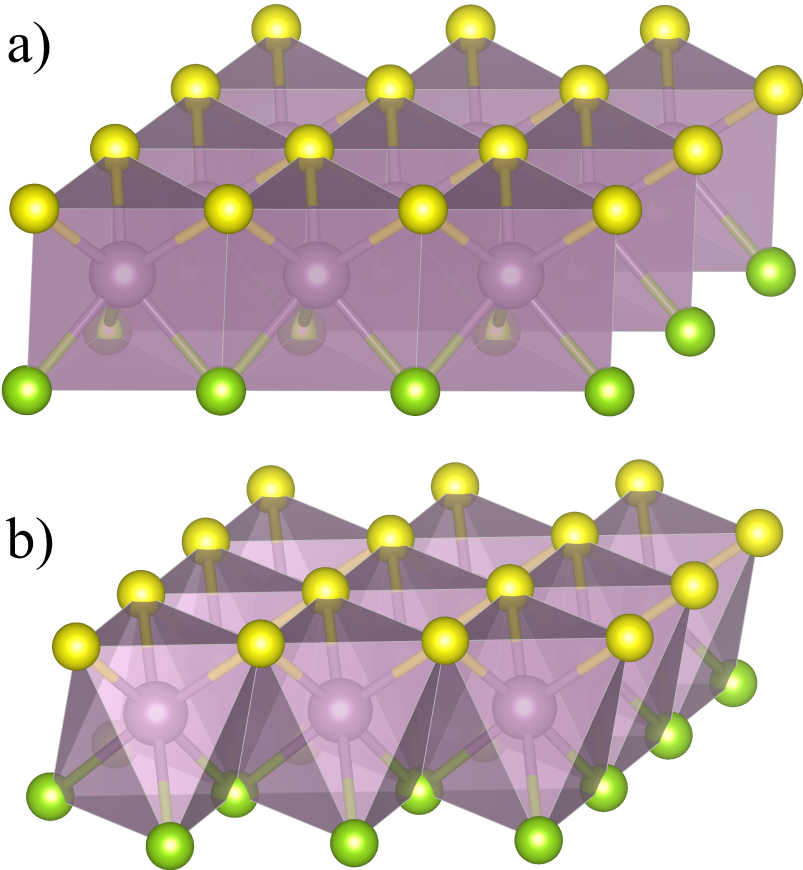
\includegraphics[width=0.4\textwidth]{1H1T.png}
        \caption{Packing of trigonal prisms and octahedra in 1H (a) and 1T (b) structures of SMoSe.}
\label{1H1T}
\end{figure}





%%%%%%%%%%%%%%%%%%%%%%%%%%%%%%%%%%%%%
		\section{Methods}
%%%%%%%%%%%%%%%%%%%%%%%%%%%%%%%%%%%%%

%%%%%%%%%
\subsection*{Crystal structure prediction}
%%%%%%%%%

The search for the lowest-enthalpy monolayer structures of SMoSe and SVSe compositions was performed using evolutionary algorithms implemented in the USPEX program package \cite{uspex1,uspex2,uspex3} and the random sampling method implemented in the AIRSS software \cite{airss1,airss2}.

The crystal structure search within USPEX was performed in fixed composition mode with 2--6 formula units per unit cell.
The number of structures in the first generation of the calculations was equal to 180.
Half of the structures with the lowest enthalpy were selected after the optimization and then used to produce the next generation.
A new generation was produced as follow: 50\% of all structures were generated by heredity, 10\% -- by atomic mutation, 10\% –- by lattice mutation, and 30\% –- randomly.
In average, 40--47 generations were produced and relaxed.
Using AIRSS program about 5000--6000 structures were randomly generated and optimized for compounds with 4 and 6 formula units per unit cell and structures with the lowest enthalpy were selected. 
In both USPEX and AIRSS calculations, to avoid adjacent layers interactions, a vacuum speparation in a direction perpendicular to the plane of the layer ($c$-axis) was set to more than 15 \AA.
 
The total energies and forces were calculated by solving the Schr\"{o}dinger equation based on projector augmented plane-wave implementation \cite{blochl1994projector} of density functional theory (DFT) using the VASP program package \cite{vasp1,vasp2}.
Exchange correlation effects were treated in the generalized gradient approximation (GGA) with Perdew-B\"{u}rke-Ernzerhof scheme \cite{pbe}.
In case of SVSe, Dudarev’s GGA+U method \cite{gga+u} with $U-J$ = 3 eV was used.
Pseudo-potentials with $4p^6 5s^1 4d^5$ (Mo), $3p^6 3d^4 4s^1$ (V), $3s^2 3p^4$ (S), and $4s^2 4p^4$ (Se) electrons have been used.

In all crystal structure prediction calculations medium-quality optimization was performed using the conjugate gradient method \cite{conjugate_gradient}. 
The energy cutoff of plane waves was set to 420 eV and 700 eV for the intermediate structures and then for the most promising of them. 
The first Brillouin zone was sampled according to Monkhorst-Pack scheme \cite{monkhorst1976special} with the density of k-point being equal to 0.5 \AA$^{-1}$ and 0.2 \AA$^{-1}$, respectively. 
The manually produced structures were optimized with the same high-quality optimization parameters.

For the test of the used methodology of crystal structure prediction, we have revealed not only the well known 1H, 1T, and 1T' structures but also recently suggested 1H' and 1S.

To study a dynamic stability of predicted structures phonon dispersion spectra were calculated within the PHONOPY code \cite{phonopy}. 
We used VESTA program for crystal structures visualization and figures preparation \cite{momma2011vesta}.
Instruments of Bilbao Crystallographic server have been used for the structures symmetrization \cite{bilbao}.



%%%%%%%%
\subsection*{Topological search}
%%%%%%%%

Within topological search, original structural information was selected from the Inorganic Crystal Structure Database (ICSD, release 2020/2) \cite{icsd_1} and Cambridge Structural Database (CSD, release 2021) \cite{icsd_2} 
\textcolor{red}{Инна, а CSD в итоге пользовались или нет? Ниже по тексту только ICSD упоминается и никаких комментариев по органике}.
In this case, the procedures of screening  by the methods of the combined geometric-topological analysis with ToposPro (http://topospro.com) package have been used \cite{topos_1}. 

We use bold three-letter symbols of the Reticular Chemistry Structure Resource nomenclature (\cite{rcsr}, http://rcsr.anu.edu.au/) or ToposPro NDk-n symbols \cite{rcsr_2}) to designate the topological types of the underlying nets
\textcolor{red}{Инна, в текущей версии у нас в одном месте используется трёх-буквенное kgd-обозначение, а топосовских последовательносей цифр нигде нет. Поэтому я предлагаю удалить вторую часть фразы}.
The topology of an underlying net was determined in an automated mode by comparison of a set of topological indices of the net with those for the reference nets from the ToposPro TTD collection \cite{TTD}.

For the topological analysis, we have used only fully solved crystal structures without errors in the determination of interatomic bonds or chemical composition.
The nets of interatomic bonds were determined by the Domains methods using the program AutoCN \cite{blatov2016_rods}. 
Only strong interatomic bonds with solid angles of the faces of Voronoi-Dirihle polyhedron ($\Omega \geq 5 $ of the whole 4$\pi$) solid angle were considered.
Structures with great values of unit cell parameters were excluded from the consideration.
For instance, we did not consider polytypes of ZnS with cell parameters more than 50 \AA.

Earlier the numerous structural relations between unhydrous simple salts and more simple binary inorganic compounds have been shown \cite{blatov2011_salts, medrish2020_zintl}. 
Due to this well-known structural phenomena, we analyse topology not only for the complete  representation, but also the topology of the underlying net.
In the complete representation, the net corresponds to the all strong interatomic bonds, while the underlying net is determined between metals and centers of ligands.
\textcolor{red}{Инна, а разве мы что-то упрощали в этом случае? Если да -- то нужно пояснить что, если нет -- то просто удалим}

Due to the short interatomic bonds, the topologies were not determined for the crystal structures 1A, 1A', 1H', and  1M''.


%%%%%%%%%%%%%%%%%%%%%%%%%%%%%%%%%%%%%
			\section{Results}
%%%%%%%%%%%%%%%%%%%%%%%%%%%%%%%%%%%%%

\subsection*{Earlier known MX$_2$ structures}

According to the performed calculations, 1H structure is the most favorable for SMoSe composition  (Table \ref{t:enthalpy}).
For SVSe composition, the most energetically favoraиle structure is 1T' (Table \ref{t:enthalpy}). 

According to our calculations, theoretically suggested 1S and 1H' \cite{tang2021_janus,ma2016_fxt} structures are characterized by the close values of enthalpies.
For both SMoSe and SVSe, 1S is more energetically favorable than 1H', with enthalpies difference equal to 0.01 ev/f.u. for SMoSe and 0.06 ev/f.u. for SVSe (Table \ref{t:enthalpy}).
Also for both SMoSe and SVSe, 1H' and 1S structures are less favorable than 1H, 1T, and 1T' structures (Table \ref{t:enthalpy}).

Another designation of 1H' and 1S structures are $fxt$ and $fes$ \cite{}\textcolor{red}{Захар, поставь ссылку где используются эти обозначения}.
In our manuscript, we use {\it 1H'} and {\it 1S}, to make the structures designation uniform.
Structurally, 1S and 1H' are different from 1T, in that in 1S and 1H' coordination polyhedra share not only common edges but also common faces (Figure \ref{fes_fxt}), which as will be shown below results in the shorter interatomic Mo--Mo bonds.
1H and 1T structures provide the most uniform distribution of the chalсogen and transition metal atoms.
Nets of both transition metal and chalcogen atoms consist of  geometrically equal triangular rings.
Edge-sharing interconnection of trigonal prisms realized in 1H' and 1S structures inevitably results in the appearance of the cavities greater in volume than the cavities of 1H and 1T. 
Cavities of 1S have the form of the slightly compressed cube (Figure \ref{fes_fxt}a).
The volume of these cavities is almost two times greater than the volume of the cavities in the 1H structure (38.8 \AA$^3$ against 17.7 \AA$^3$ for SMoSe).
The volume of hexagonal cavities of 1H' structure (Figure \ref{fes_fxt}b is almost 8 times greater than the volume of cavities in 1H (137.8 \AA\ against 17.7 \AA$^3$ for SMoSe).

In contrast to trigonal prisms, the face-sharing of the octahedra seems to be problematic for quasi 2D structure, as it results in the deviation from the flat arrangement.
However, as it will be shown below, the dynamically stable quasi-2D structure characterized by the face-sharing of octahedra was also predicted.



%%%%%%%%%%%%%%%%%%%%%%%%%%%%%%%%%%%%%
		\subsection{New structures}
%%%%%%%%%%%%%%%%%%%%%%%%%%%%%%%%%%%%%

New crystal structures were produced in two different ways, in an automated manner by USPEX or AIRSS, and manually -- based on the 1H structure.

The new structures are characterized by triclinic, monocliniс, or orthorhombic symmetry.
We will designate them as 1A, 1M, and 1O, respectively
To differentiate structures of the same symmetry we will use single quotes.
For instance, {\it 1A, 1A', 1A''}, and {\it 1A'''} are the crystal structures of triclinic symmetry, with sufficiently different atomic arrangements.


%%%%%%%%%%%%%%%%%%%%%%%%
\subsubsection{Structures revealed with {\it unbiased} algorithms}
%%%%%%%%%%%%%%%%%%%%%%%
Table \ref{t:enthalpy} shows the values of the predicted structures, figures \ref{phon_svse} and  \ref{phon_smose} -- their phonon dispersion curves. 

Among the found structures, 1M-SVSe and 1A'-SMoSe are the most promising ones.
In addition to dynamic stability, the enthalpies of formation of 1A'-SMoSe and 1M-SVSe are lower than that of 1T of the same composition. 

For SMoSe composition, crystal structures 1M', 1A''',and 1M'' are dynamically stable, but energetically less favorable than 1H or 1T (Figure \ref{phon_smose}, Table \ref{t:enthalpy}).
For SVSe composition, 1A and 1A'' are dynamically stable (Figure \ref{phon_svse}). 

Below we describe the revealed crystal structures, beginning from the most energetically favorable ones.
To simplify description of the structural relations between numerous revealed structures, below we show in pairs crystal structures, produced by optimization of the same structure.
These structures will be described together.
The dynamically stable structures are highlighted in bold, only these structures will be further considered.

\begin{tabbing} \centering
	AAAAAAAAAA \= AAAAAAAAA \kill
	{\bf 1M-SVSe} \> 1M-SMoSe \\
	1M'-SVSe \> {\bf 1M'-SMoSe} \\
	{\bf 1A-SVSe} \> {\bf 1A'-SMoSe} \\
	{\bf 1A''-SVSe} \> {\bf 1A'''-SMoSe} \\
	
	1O-SVSe \> {\bf 1O-SMoSe} \\
	1O'-SVSe \> 1O'-SMoSe \\
	1M''-SVSe \> {\bf 1M''-SMoSe}
\end{tabbing}

\begin{table}[H]
	\caption{Calculated enthalpies of SMoSe and SVSe structures produced using crystal structure prediction techniques.} \label{t:enthalpy} \vspace{2mm}
	\centering
	\begin{tabular}{l*{5}{l}}
		\hline \hline
		\multirow{2}*{Phase} & \multicolumn{2}{c}{Enthalpy (eV/f.u.)} & \multicolumn{2}{c}{Relative H (eV/f.u.)}	\\
		\cline{2-3} \cline{4-5}
		& SMoSe & SVSe & SMoSe & SVSe\\
		\hline    		
		1H	    &	-20.8588	&	-15.7908	&	0.0000	&	0.2022	\\
		1T  	&	-20.1229	&	-15.8817	&	0.7358	&	0.1113	\\
		1T' 	&	-20.4272	&	-15.9930	&	0.4315	&	0.0000	\\
		1S   	&	-20.0677	&	-15.3545	&	0.7910	&	0.6385	\\
		1H' 	&	-20.0572	&	-15.2915	&	0.8016	&	0.7015	\\
		1M  	&	-20.3004	&	-15.9091	&	0.5584	&	0.0838	\\
		1M'  	&	-20.0648	&	-15.7256	&	0.7939	&	0.2674	\\
		1A, 1A'		&	-20.2308	&	-15.6641	&	0.6280	&	0.3289	\\
		1A'', 1A'''	&	-19.6106    &	-15.6467	&	1.2481 	&	0.3463	\\
		1O  	&	-19.7876	&	-15.2359	&	1.0711	&	0.7571	\\
		1O'	    &	-20.2611	&	-15.4713	&	0.5977	&	0.5217	\\
		1M''    &	-19.9359	&	-15.5461	&	0.9229	&	0.4468	\\
		\hline \hline
	\end{tabular}
\end{table}


\begin{figure}[H]
	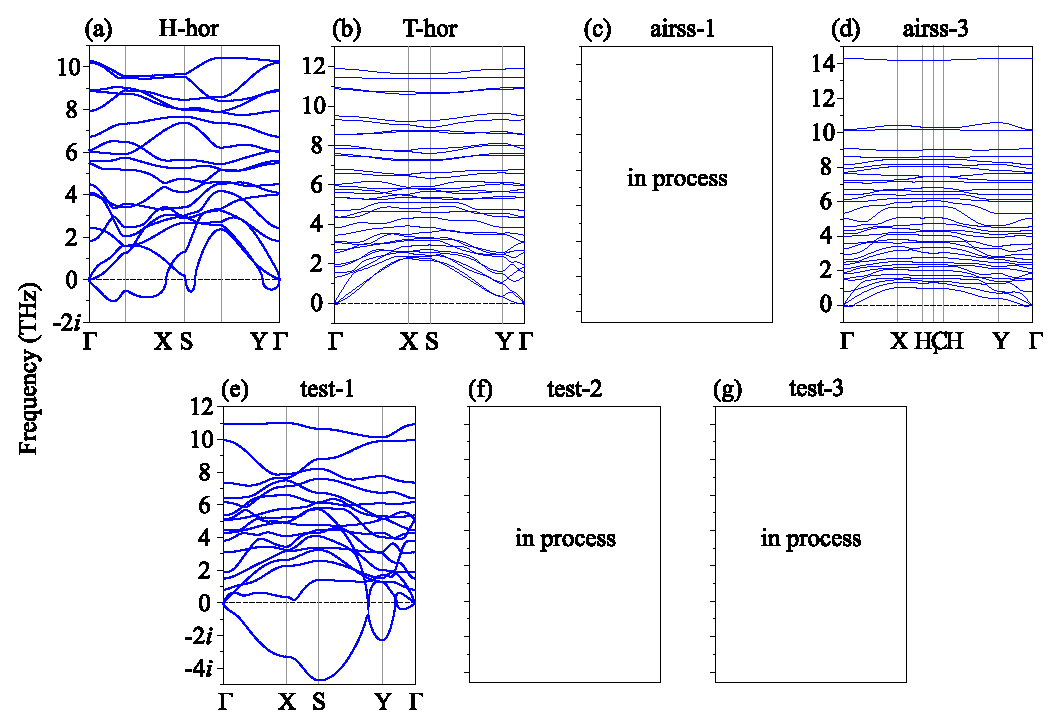
\includegraphics[width=\textwidth]{phon_svse.eps}
	\caption{Phonon dispersion curves of SVSe structures.}
	\label{phon_svse}
\end{figure}


\begin{figure}[H]
	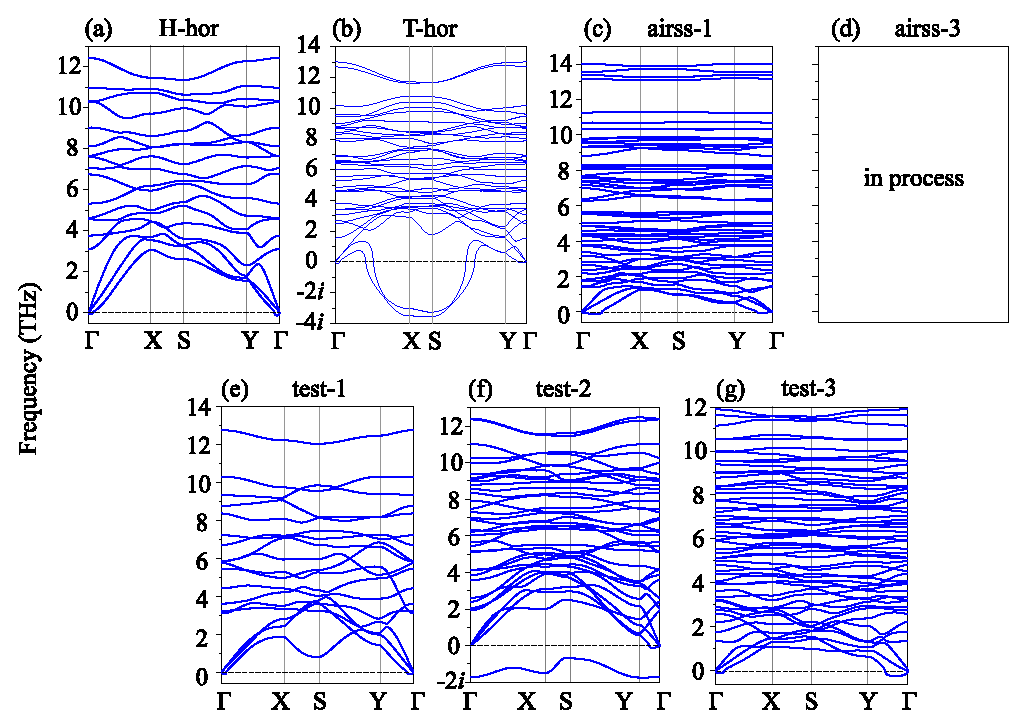
\includegraphics[width=\textwidth]{phon_smose.eps}
	\caption{Phonon dispersion curves of SMoSe structures.}
	\label{phon_smose}
\end{figure}







\paragraph{1M-SVSe}

The structure with monoclinic symmetry was predicted using USPEX for SVSe and was called 1M-SVSe. 
For SVSe composition it is more  energeticaly favorable than both 1H and 1T structures, although it is less favorable than 1T' (Table \ref{t:enthalpy}).
Calculation of phonon dispersion curves have shown dynamic stability of SVSe-1M (Figure \ref{phon_svse}) and instability of SMoSe-1M (Figure \ref{phon_smose}).

1M structure is characterized by the same octahedral coordination polyhedron as 1T structure.
The difference is in the arrangement of the coordination [TMSSe$_3$] octahedra.
As it was mentioned, in 1T structure octahedra share only common edges, while in 1M edges and faces.
Both structures can be described within a modular approach.
In this case, 1T and 1M structures can be restored from the same structural module.
The module is the double row of octahedra, connected through the common edges.
In Figure \ref{T_hor_T} one of such double rows is the row consisting of the rows \# 2 and \# 3.
In the 1M structure, the adjacent double rows are attached through the common faces  of the octahedra (the face I(II)III on the Figure \ref{T_hor_T}).
In the 1T structure, the interconnection of double rows is edge-sharing (the edge II'III' in Figure \ref{T_hor_T}). 
The comparison of these two types of interconnection is shown in Figure \ref{T_hor_slabs}.


The presence of common faces of coordination octahedra results in the formation of shorter V--V bonds, forming the zig-zag chains of V atoms (Figure \ref{T_hor_V}).
This in turn results in the undulation of the whole structure (Figures \ref{T_hor_hcb}).
The nets sulphur and chalcogen atoms in 1M structure it is topologically the same as that in 1T structure, although sufficiently deformed (Figure \ref{T_hor_hcb}).
The angles between S--S bonds in SVSe-1M structure vary in the range 91.38-139.8\textdegree, while in 1T structure all the angles are equal to 120\textdegree (Figure \ref{T_hor_ch}).
The S--S bond lengths in 1M are in the range 3.45--3.87\AA, while in SVSe-1T all they are equal to 3.41 \AA (Figure \ref{T_hor_ch}).


\begin{figure}[H]
	\includegraphics[width=0.8\textwidth]{T_hor_T.png} \\
	\caption{Comparison of 1M and 1T crystal structures.}
	\label{T_hor_T}
\end{figure}

\begin{figure}[H]
	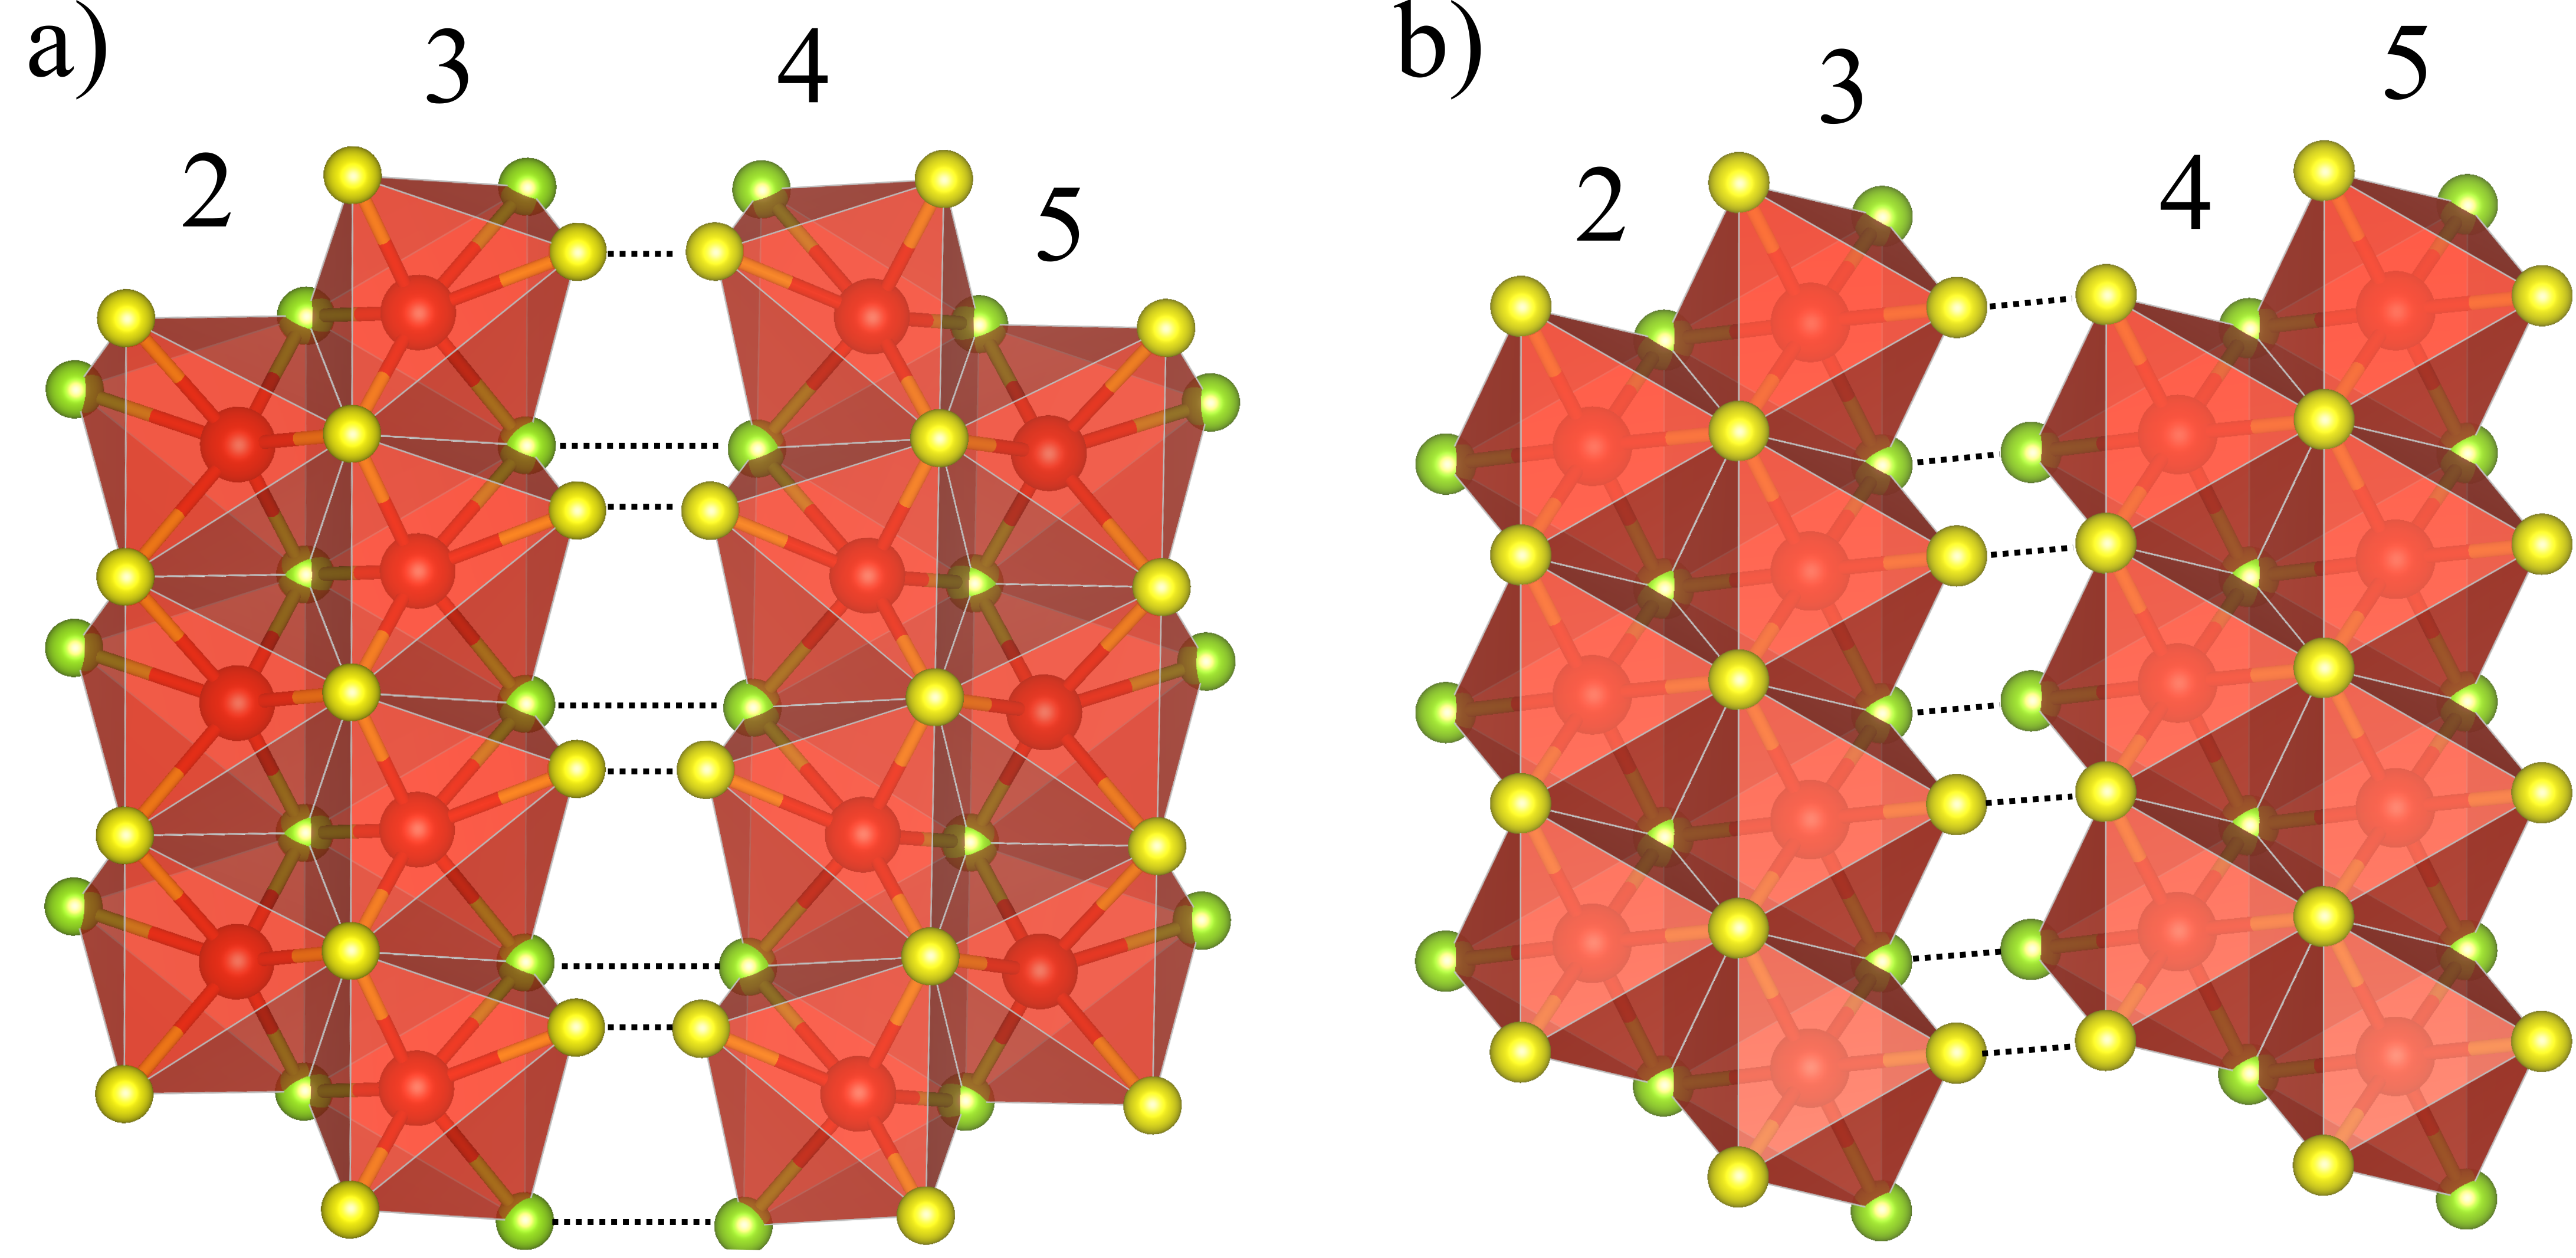
\includegraphics[width=0.7\textwidth]{T_hor_slabs.png} \\
	\caption{Arrangement of double octahedral rows in 1M (a) and 1T (b) structures; the dashed lines show the common atoms in the adjacent slabs.}
	\label{T_hor_slabs}
\end{figure}


\begin{figure}[H]
	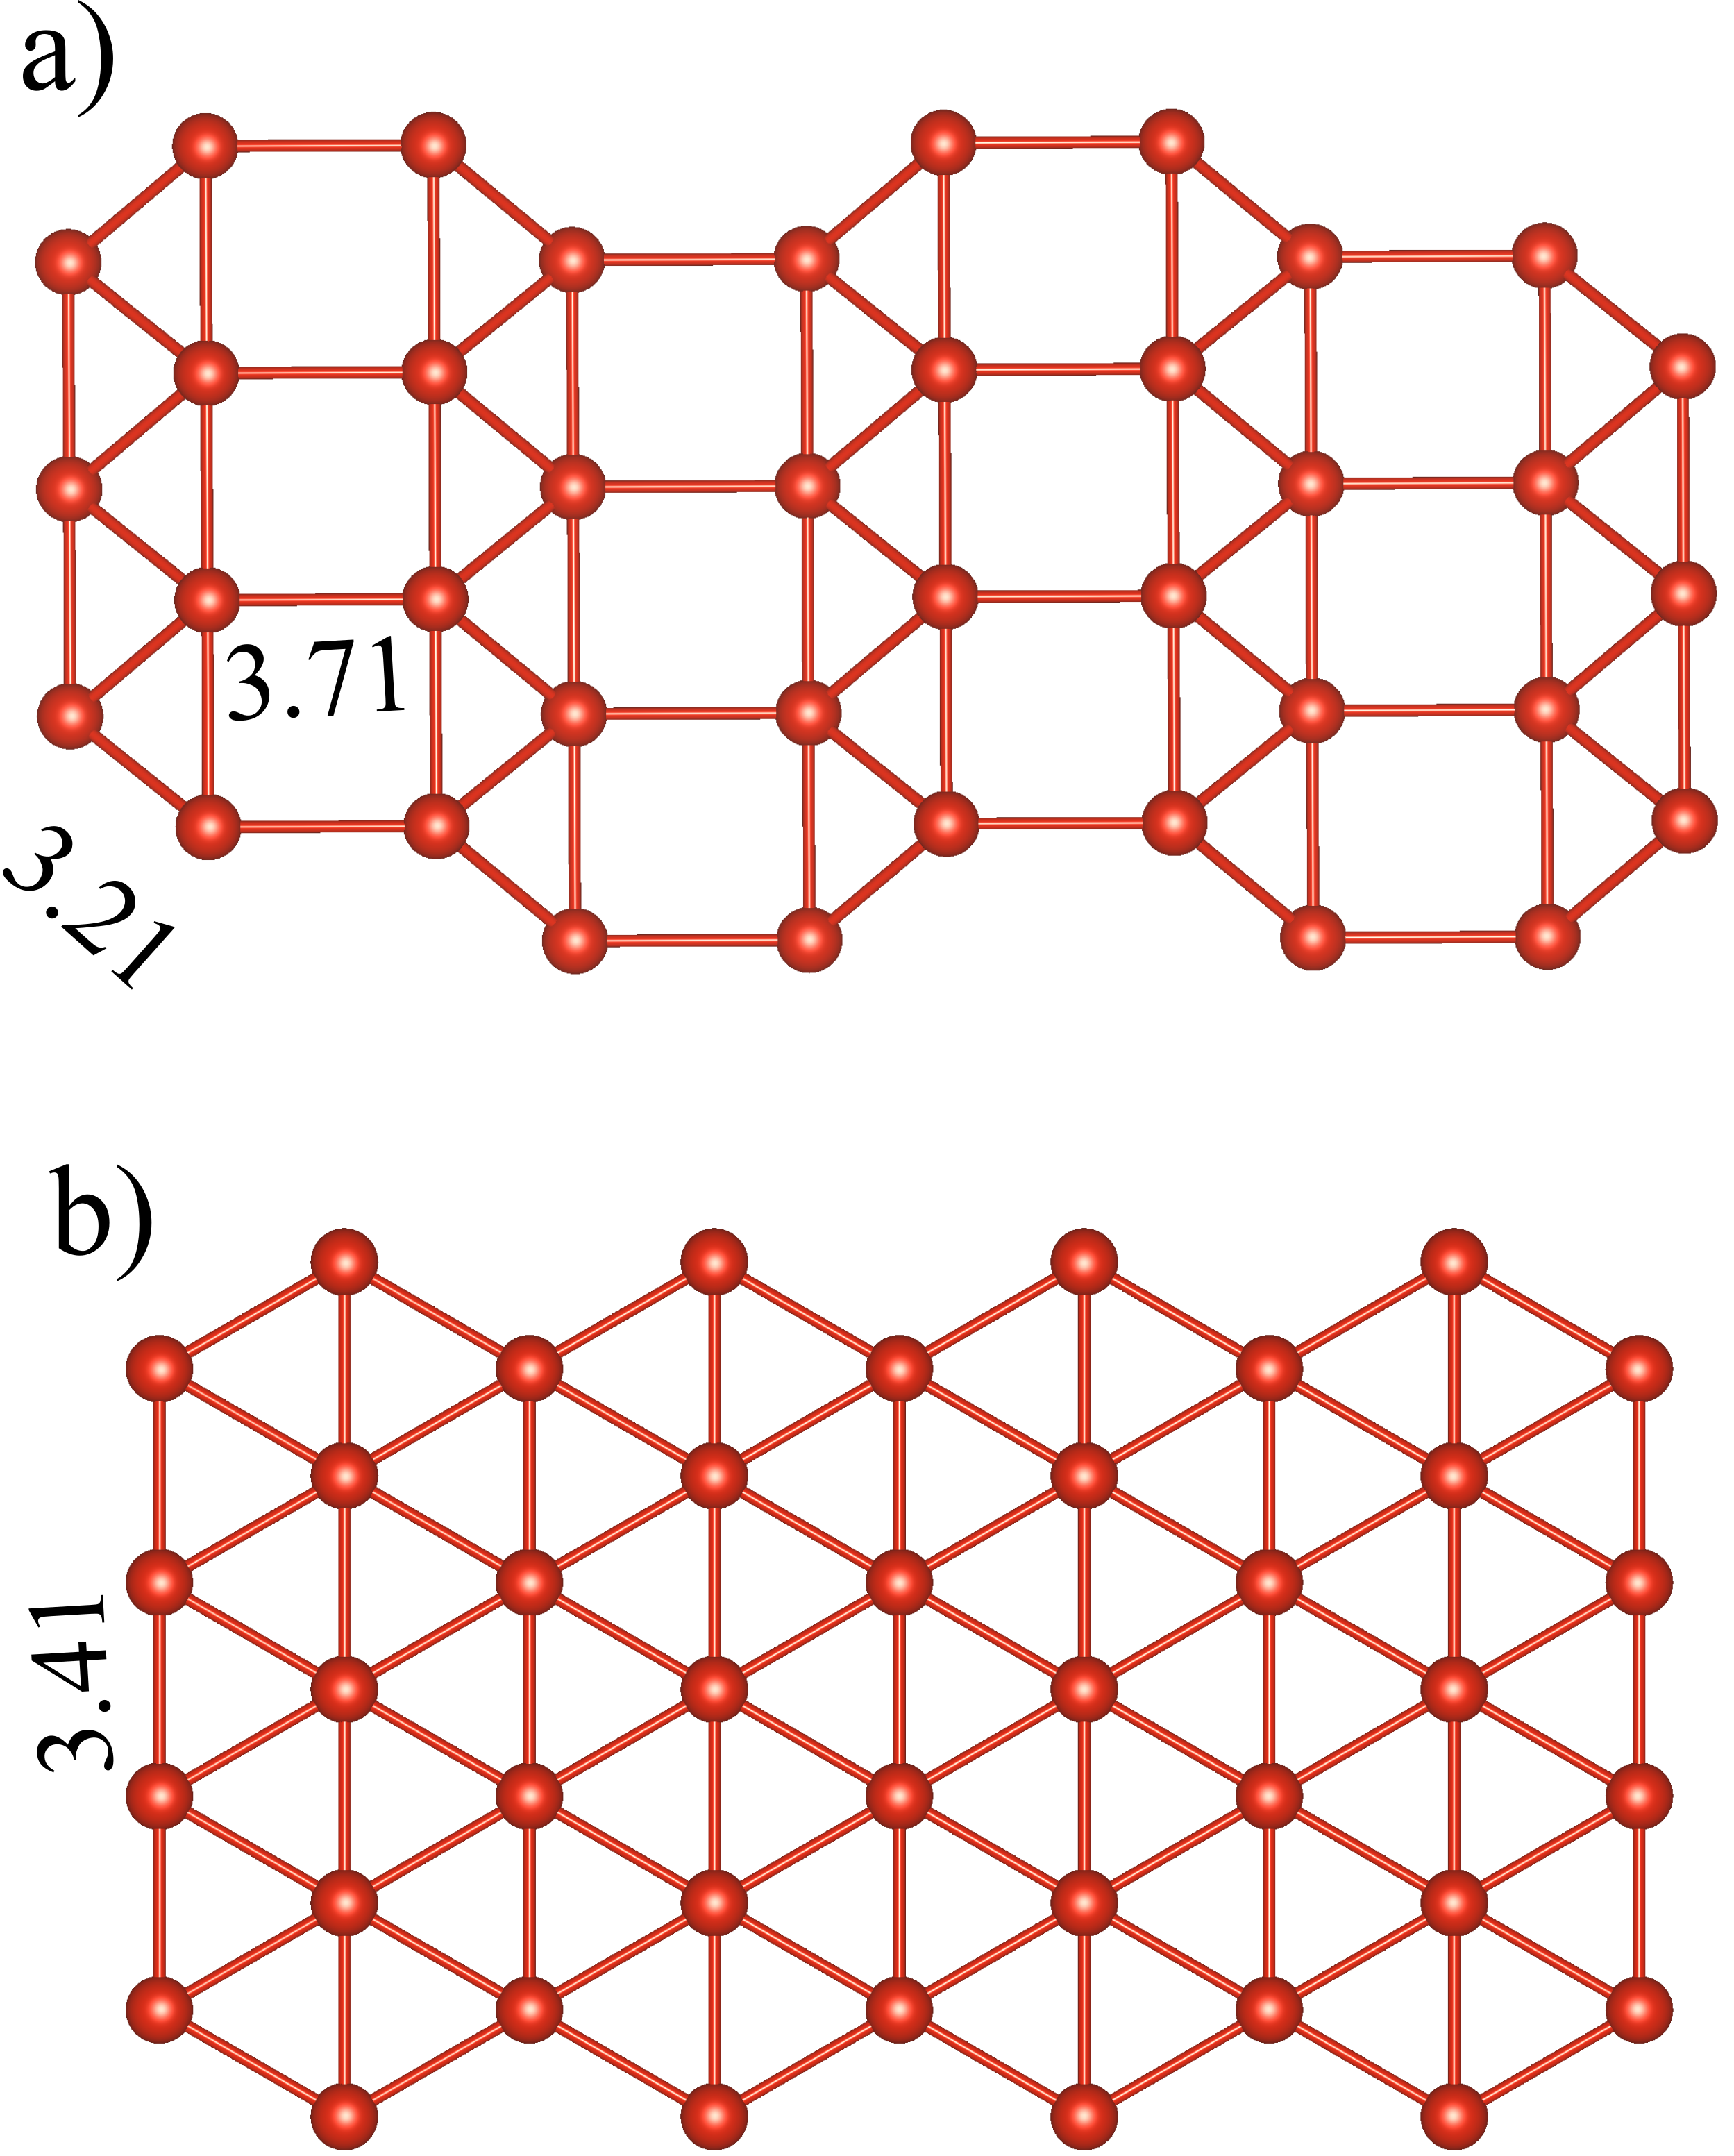
\includegraphics[width=0.4\textwidth]{T_hor_V.png} \\
	\caption{Comparison of the nets of TM atoms in 1M (a) and 1T (b) crystal structures; values of interatomic distances are given in \AA.}
	\label{T_hor_V}
\end{figure}

\begin{figure}[H]
        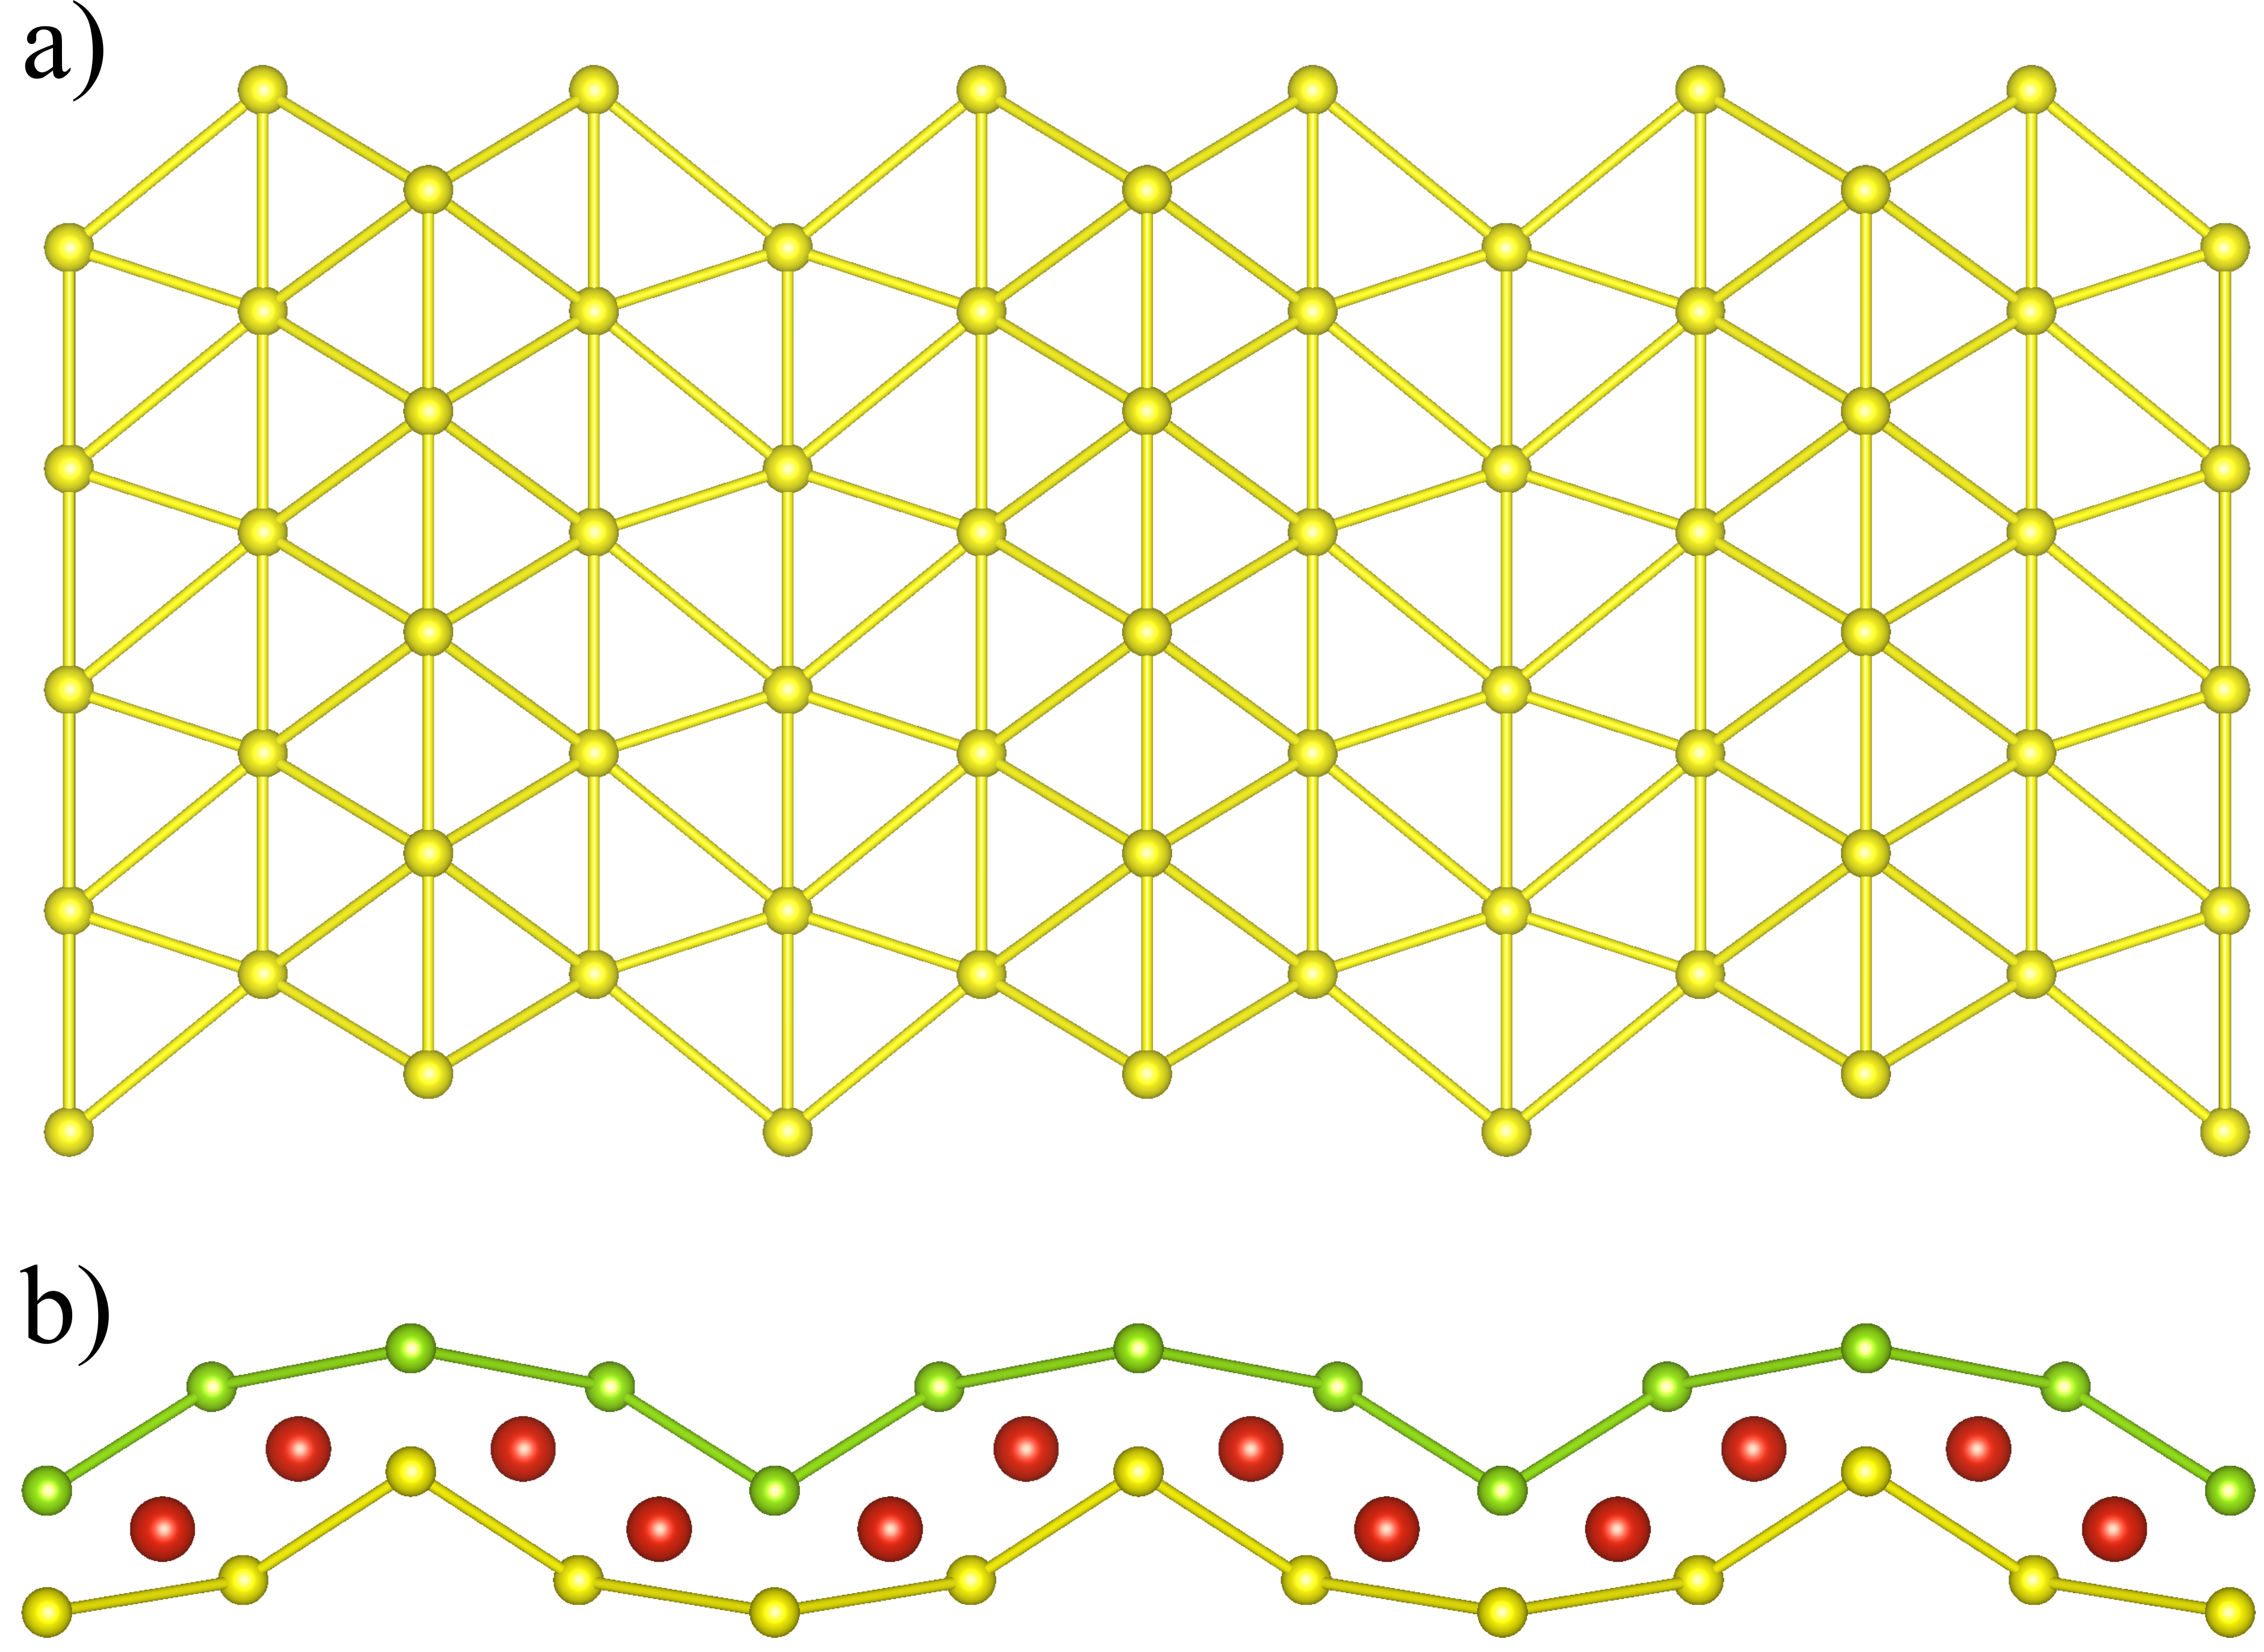
\includegraphics[width=0.5\textwidth]{T_hor_hcb.png} \\
        \caption{The undulated net of chalcogen atom in 1M structure: top- (a) and side-view (b); sulphur is shown in yellow, selenium -- in green, vanadium -- in red.}
\label{T_hor_hcb}
\end{figure}



\paragraph{1M'-SMoSe}
Another structure with monoclinic symmetry sufficiently different from 1M was found using the USPEX package for SMoSe composition.
This structure was named SMoSe-1M'.
1M' structure is dynamically stable for SMoSe (Figure \ref{phon_smose}) and unstable for SVSe (Figure \ref{phon_svse}).

Enthalpy of SMoSe-1M' is higher than the enthalpy of SMoSe-1T on 0.05 eV/f.u. (Table \ref{t:str})

1M' structure is different from the other structures in that it is characterized by the almost right square net of chalcogen atoms (Figure \ref{H-hor}).
The bottom (selenium) layer is shifted relatively to top (sulfur) one (Figure \ref{H-hor}).
Transition metal atoms are arranged in such a way to have trigonal prismatic coordination.
Similarly, as it is in 1H, in 1M' structure trigonal prisms share only common edges, but not common faces.
Molybdenum atoms are connected by the bonds of 3.08--3.22 \AA\ lengths in quasi-1D chains (Figure \ref{H-hor_Mo}).
The chains are connected by the sufficiently weaker bonds of 4.08 \AA\ length (Figure \ref{H-hor_Mo}).


\begin{figure}[H]
	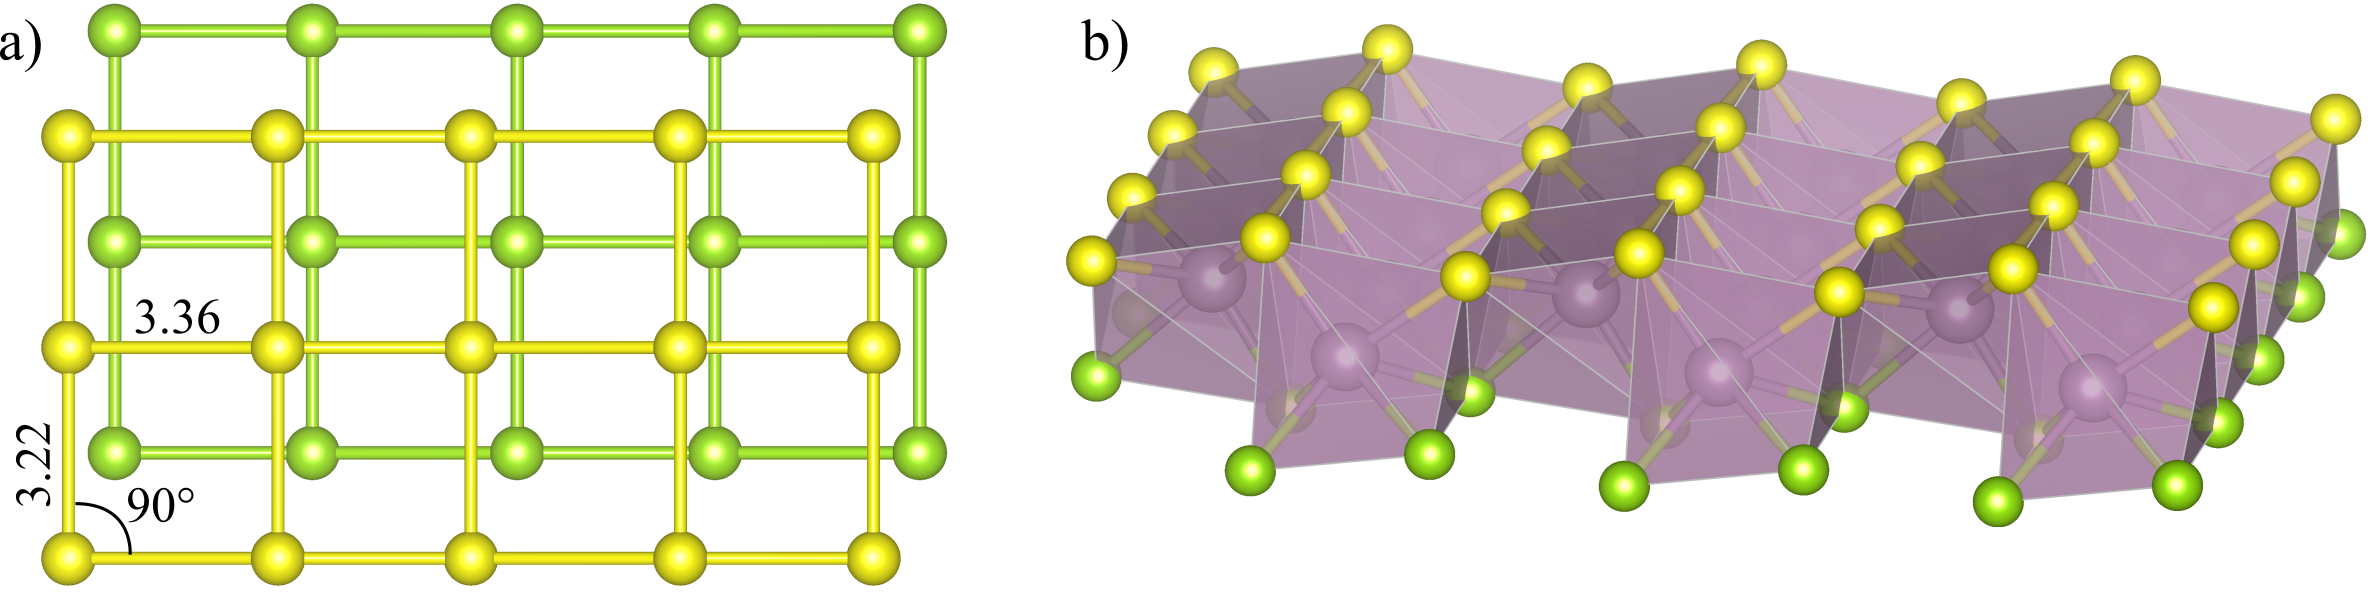
\includegraphics[width=\textwidth]{H-hor.png}
	\caption{Nets of sulfur (yellow) and selenium (green) atoms (a) and arrangement of coordination polyhedra around Mo atoms (b) in 1M'-SMoSe.}
	\label{H-hor}
\end{figure} 


\begin{figure}[H]
	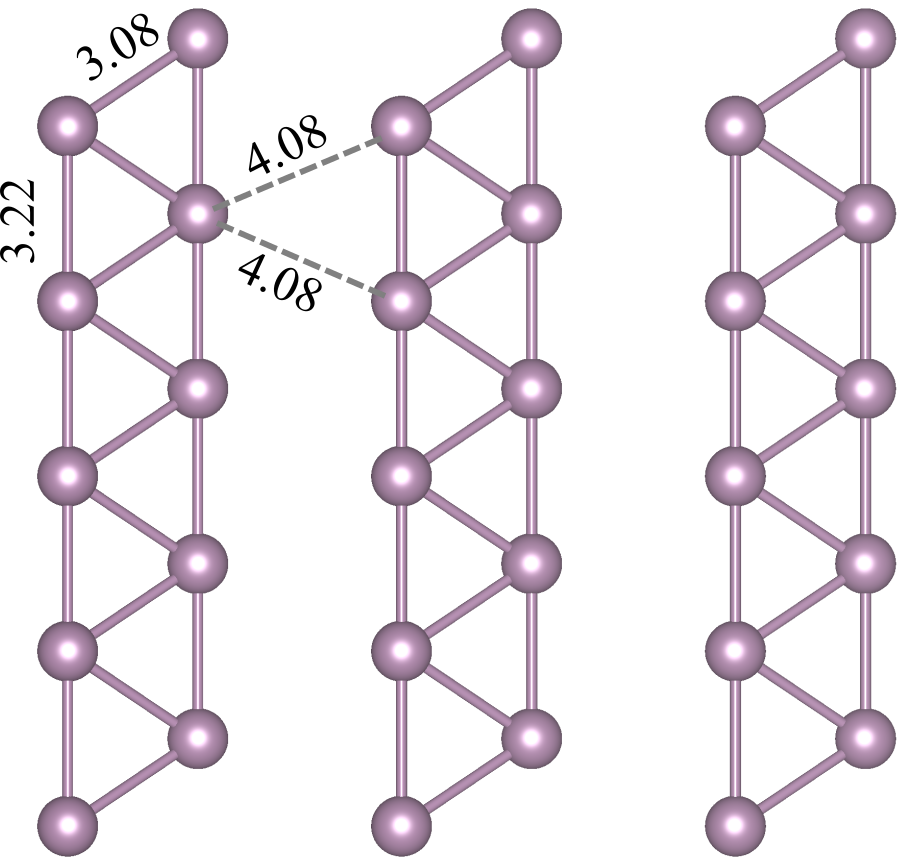
\includegraphics[width=0.4\textwidth]{H-hor_Mo.png}
	\caption{Chains of molybdenum atoms in SMoSe-1M'.}
	\label{H-hor_Mo}
\end{figure} 


\paragraph{1A-SVSe and 1A'-SMoSe}
The structure with triclinic symmetry called 1A', was revealed with AIRSS package for SVSe composition.
Despite sufficient structural similarity between optimized 1A structure for SMoSe and SVSe compositions, there is an apparent crystallographic difference between them, similar to that observed for 1T and 1T'.
Based on this we will designate them as 1A-SVSe and 1A'-SMoSe.
Both 1A-SVSe and 1A'-SMoSe are dynamically stable (Figures \ref{phon_smose} and \ref{phon_svse}).

The enthalpy of 1A'-SVSe structure lies in-between values of enthalpies of 1T and 1T' structures, being more favorable than 1T on nearly 0.1 eV/f.u.
The enthalpy ratio for SMoSe composition is the following: 
$H(1H) < H(1T') < H(1A) < H (1T)$.
For SVSe composition, 1A is less favorbale than 1T', 1T, and 1H structures (Table \ref{t:enthalpy}).


The structures 1A and 1A' can be better described based on the net of TM atoms, which forms the well known kagome lattice\cite{zhang2021_kagome}, observed for instance in AV$_3$Sb$_5$ \cite{ortiz2021} and WO$_3$ \cite{gerand1979} compounds.
In 1A-SVSe and 1A'-SMoSe, kagome lattices are not of ideal hexagonal symmetry, there is the dispersion of bond lengths and deviation of bond angles from ideal values of 120\textdegree.
In 1A'-SVSe, the bond lengths vary in the range 3.07--3.49 \AA\ and bond angles –- in the rage 115-122.9\textdegree\ (Figure \ref{airss1_tm}a).
In 1A'-SMoSe, the bond lengths are in the wide range of 2.78--3.79 \AA, and bond angles are in the range 113.9--125.7\textdegree\ (Figure \ref{airss1_tm}b).
1A'-SMoSe is different from 1A-SVSe in that it is characterized by the presence of triangular clusters of TM atoms with sufficiently shorter bond lengths.
The bond lengths within clusters are equal to 2.78--2.81 \AA, while other Mo--Mo bonds are on 0.5--1 \AA\ longer (Figure \ref{airss1_tm}b).
In SMoSe-1T', the zig-zag chains of Mo atoms are connected by the bond of 2.79 \AA\ length, i.e. they are equal to the bond lengths within triangular clusters.
As it will be shown below, the formation of clusters and chains of molybdenum atoms are typical for the revealed structures.

The nets of sulfur atoms in 1A and 1A' structures are different from that in 1T or 1H structures (Figure \ref{airss1_s}) but similar to each other (Figure \ref{airss1_s_comp}).
Sulfur net of 1A can be transformed into the sulfur net of 1H (or 1T) by the shift, shown in Figure \ref{airss1_s} and subsequent deformations.
Differences of bond angles and bonds lengths in 1A and 1A' structures do not exceed 0.1 \AA\ and 1\textdegree.
The net of sulfur atom is not planar, the deviation from the planar arrangement is nearly equal to $\pm$10\textdegree.

In 1A and 1A' structures, each transition metal atom is coordinated by chalcogen atoms arranged in highly deformed tetragonal pyramids.
The composition of such pyramids are (TM)S$_3$Se$_2$ or (TM)S$_2$Se$_3$.
The bond distances between TM and Ch atoms vary in the range 2.26--2.58 \AA\ for 1A-SVSe and in the range 2.29--2.63 \AA\ for 1A'-SMoSe.
The pyramids are grouped in three, forming triangles of TM atoms.
These triangles correspond to the triangular rings of kagome lattice (Figure \ref{airss1_poly}).
Between triangular clusters of TM atoms, there are the big holes -- the hexagonal rings of kagome lattice \ref{airss1_poly}).



\begin{figure}
	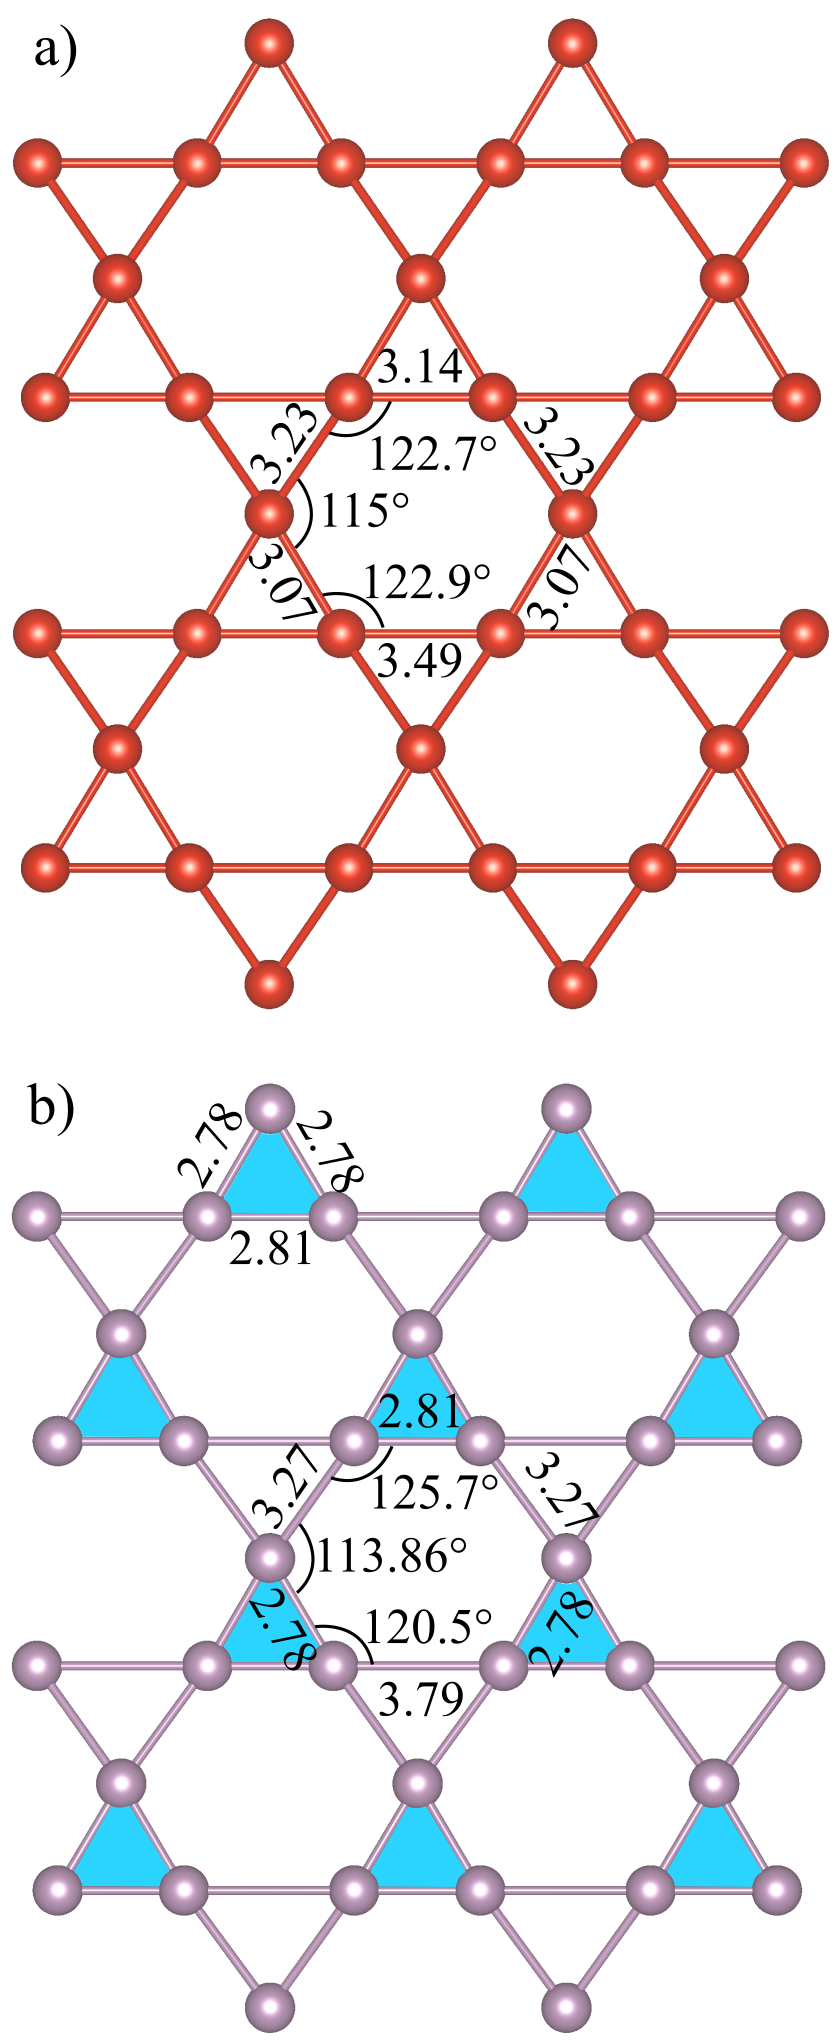
\includegraphics [width=0.35\textwidth]{airss1_tm.png}
	\caption{The kagome atomic nets of transition metal atoms in 1A'-SVSe (a) and SMoSe-1A (b); triangular clusters of Mo atoms are highlighted in blue.} 
\label{airss1_tm}
\end{figure}

\begin{figure}
	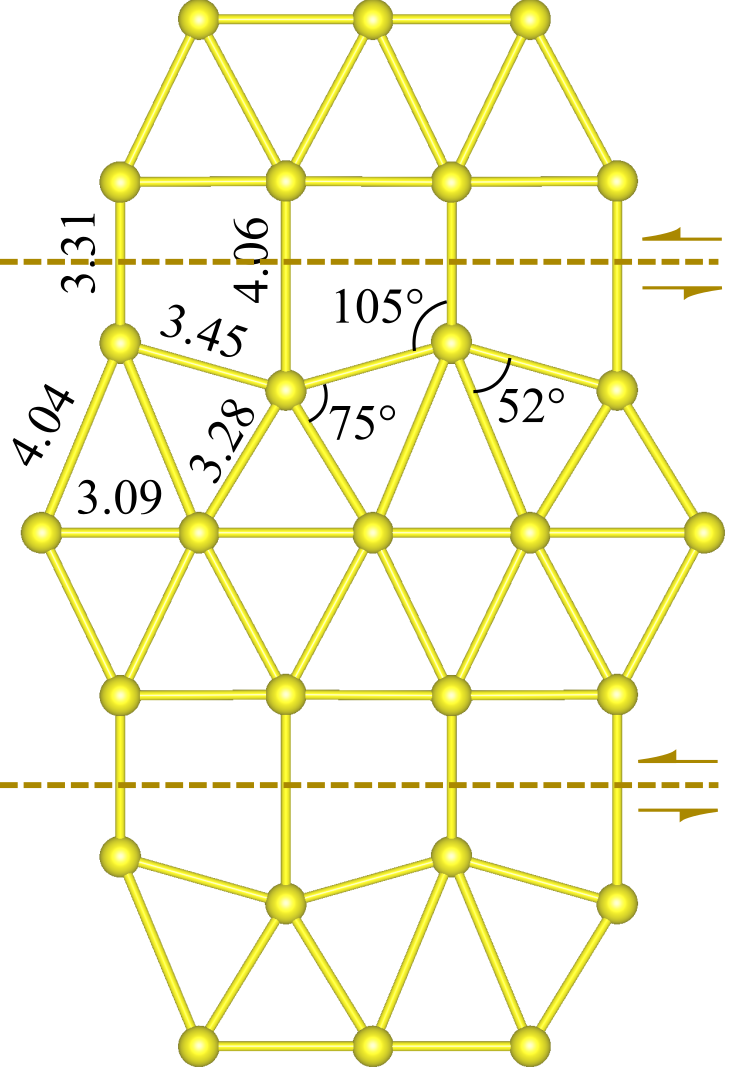
\includegraphics[width=0.35\textwidth]{airss1v_s.png}
	\caption{Net of sulfur atoms in 1A-SVSe; dashed lines show the plane of the shift transforming the net into the hexagonal one of 1T and 1H structures.}
\label{airss1_s}
\end{figure}


\begin{figure}[H]
        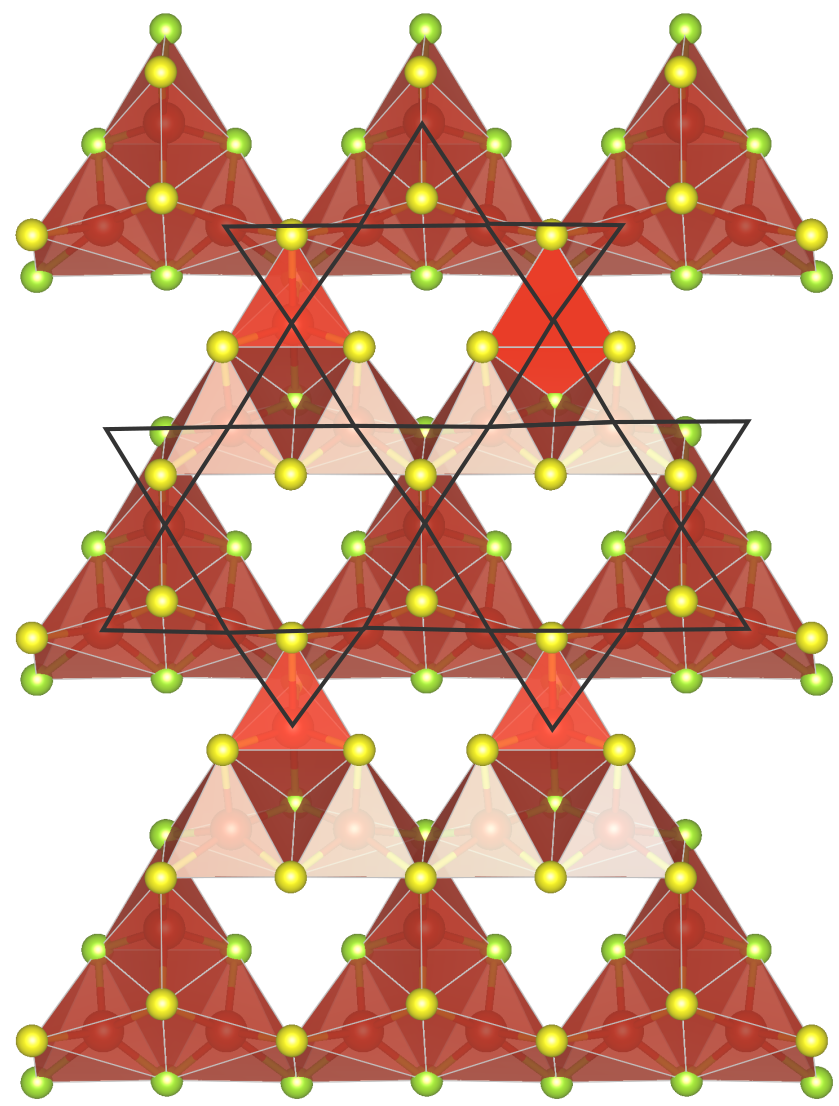
\includegraphics[width=0.35\textwidth]{airss1_v_poly.png}
        \caption{1A-SVSe with outlined coordination polyhedra around V atoms; kagome lattice is outlined in black.}
\label{airss1_poly}
\end{figure}




\paragraph{1A''-SVSe and 1A'''-SMoSe}
One more crystal structure with triclinic symmetry was revealed for SVSe composition using AIRSS code and them optimized for SMoSe composition.
There are drastic differences between optimized SMoSe and SVSe structures and we will designate them as 1A''-SVSe and 1A'''-SMoSe.

Crystal structures  1A-SVSe and 1A'''-SMoSe give the visual illustration for the different effects of vanadium and molybdenum atoms on the crystal structure of TMDs.
Both structures are dynamically stable (Figures \ref{phon_smose} and \ref{phon_svse}).
Enthalpies of the 1A'' and 1A''' structures are higher than the enthalpies of 1H, 1T, and 1T' of the same composition (Table \ref{t:enthalpy}).
1A''-SVSe is more favorable than 1S and 1H' structures on nearly 0.4 eV/f.u., while 1A'''-SMoSe is less favorable on the same value of energy (Table \ref{t:enthalpy}).

Differences of 1A'' and 1A''' can be clearly seen in the side-view.
In 1A''-SVSe, TM atoms are nearly in the same plane as Ch atoms, while in 1A'''-SMoSe,  they are in-between the layers of Ch atoms.

The nets of chalcogen atoms are also sufficiently different.
In 1A''-SVSe, the topology of the net corresponds to the graphite-like hexagonal net, while in 1A'''-SMoSe chalcogen atoms form a triangular net, if the weak contacts of 4.58-4.64 \AA\ are considered.
The new crystal-chemical feature of 1A''-SVSe which was not observed for the other TMDs structures is the presence of S--S and Se--Se dimers with the bond length of 2.09 \AA\ and 2.37 \AA, respectively (Figures \ref{airss3_svse}a and \ref{airss3_S_Se}).
These bond lengths correspond to that in the crystals structures of elemental sulfur and selenium.
Other S--S and Se--Se bonds of 1A''-SVSe are  sufficiently longer, varying in the range 3.17--3.73 \AA\ (Figures \ref{airss3_svse}a and \ref{airss3_S_Se}).
In 1A'''-SMoSe there are no clusters of Ch atoms, S--S bonds vary in the range 3.24-3.79 \AA\ with the weak contacts of 4.58--4.64 \AA\ (Figure \ref{airss3_svse}a).

The nets of TM atoms in 1A'' and 1A''' are also drastically different, as it is illustrated in the Figures \ref{airss3_svse}b and \ref{airss3_smose}b.
1A'''-SMoSe is characterized by the presence of Mo--Mo dimers with the bond lengths of 2.85 \AA, while other bonds vary in the range 3.04--3.74 \AA\ (Figure \ref{airss3_smose}b).
There are no such short bonds in 1A''-SVSe, in which V--V bonds smoothly vary in the range 3.32--3.79 \AA.

TM atoms in 1A''-SVSe are five and six-coordinated by Ch atoms (Figure \ref{airss3_poly}a);
coordination polyhedra are  deformed tetragonal pyramid and trigonal prism, respectively.
1A'''-SMoSe is characterized by the lower coordination numbers.
Vanadium atoms in it are four- and five-coordinated; coordination polyhedra -- deformed tetrahedron and trigonal bipyramid, respectively (Figure \ref{airss3_poly}b).
1A''-SVSe is characterized by the infinite quadruple chains of coordination polyhedra (Figure \ref{airss3_poly}a) and 1A'''-SMoSe -- by the signle chains (Figure \ref{airss3_poly}b).
In both structures, coordination polyhedra in the chains are connected through the common edges (Figure \ref{airss3_poly}).
The adjacent chains in 1A''-SVSe are connected through the common edges, while in 1A'''-SMoSe -- through the common vertices (Figure \ref{airss3_poly}).

\begin{figure}[H]
	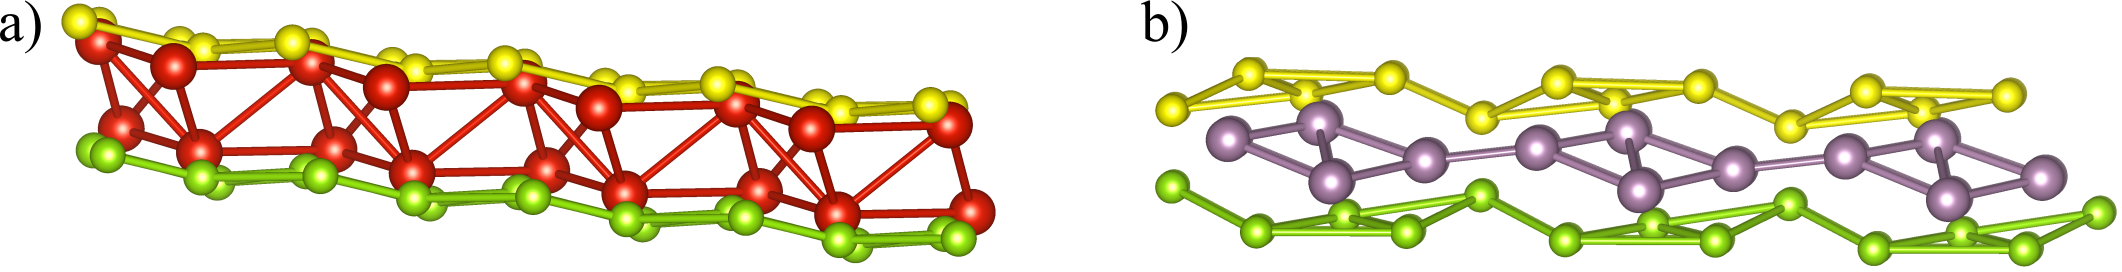
\includegraphics[width=\textwidth]{airss3_side.png}
	\caption{The side-view of 1A''-SVSe (a) and 1A'''-SMoSe (b) structures.}
	\label{airss3_side}
\end{figure}

\begin{figure}[H]
	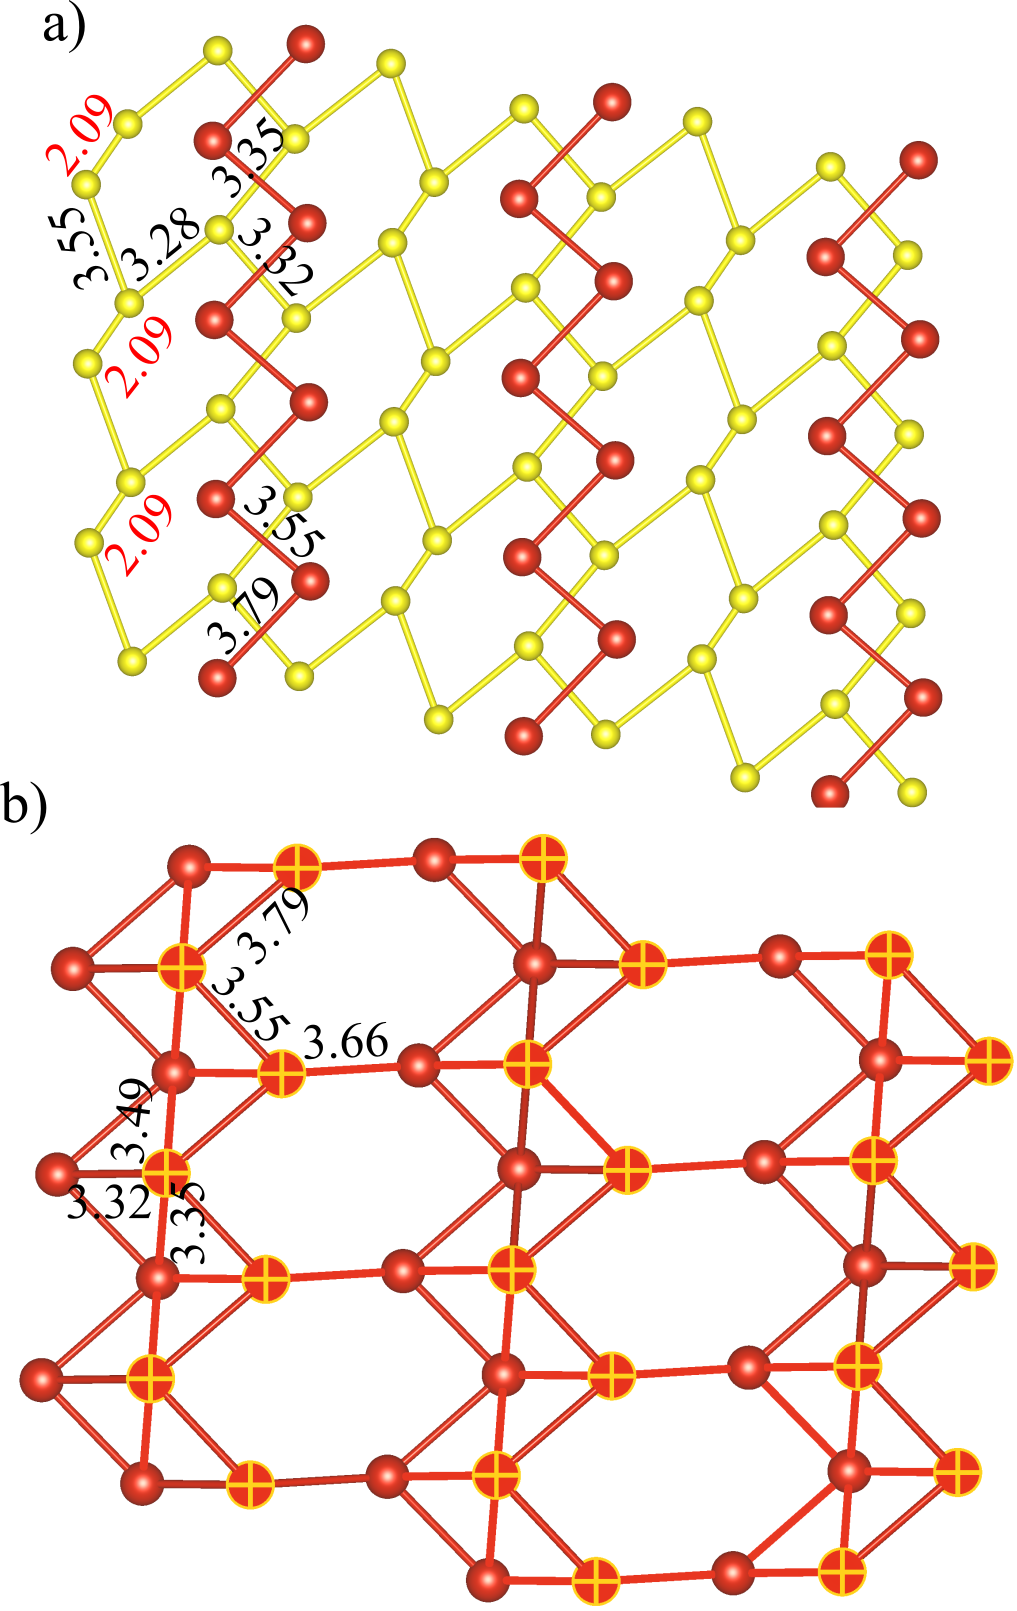
\includegraphics[width=0.5\textwidth]{airss3_svse.png}
	\caption{The nets of sulfur (a) and vanadium (b) atoms in 1A''-SVSe; vanadium atoms of the upper layer are highlighted.}
	\label{airss3_svse}
\end{figure}

\begin{figure}[H]
	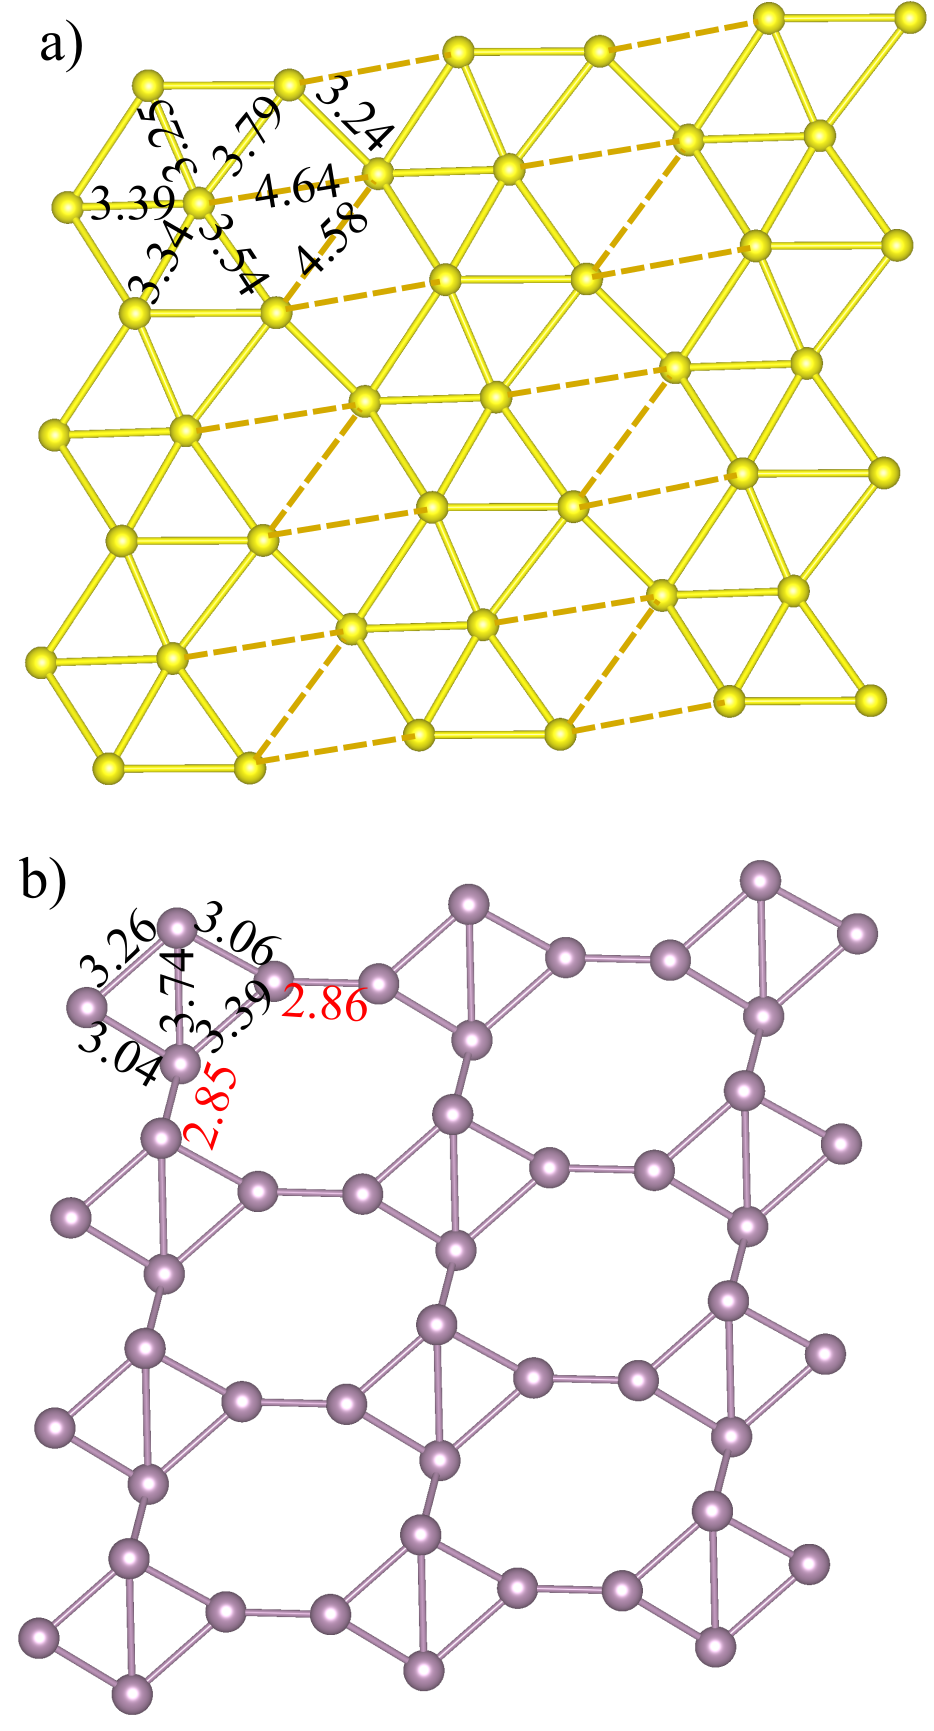
\includegraphics[width=0.5\textwidth]{airss3_smose.png}
	\caption{The nets of sulfur (a) and molybdenum (b) atoms in 1A'''-SMoSe.}
	\label{airss3_smose}
\end{figure}


\begin{figure}[H]
	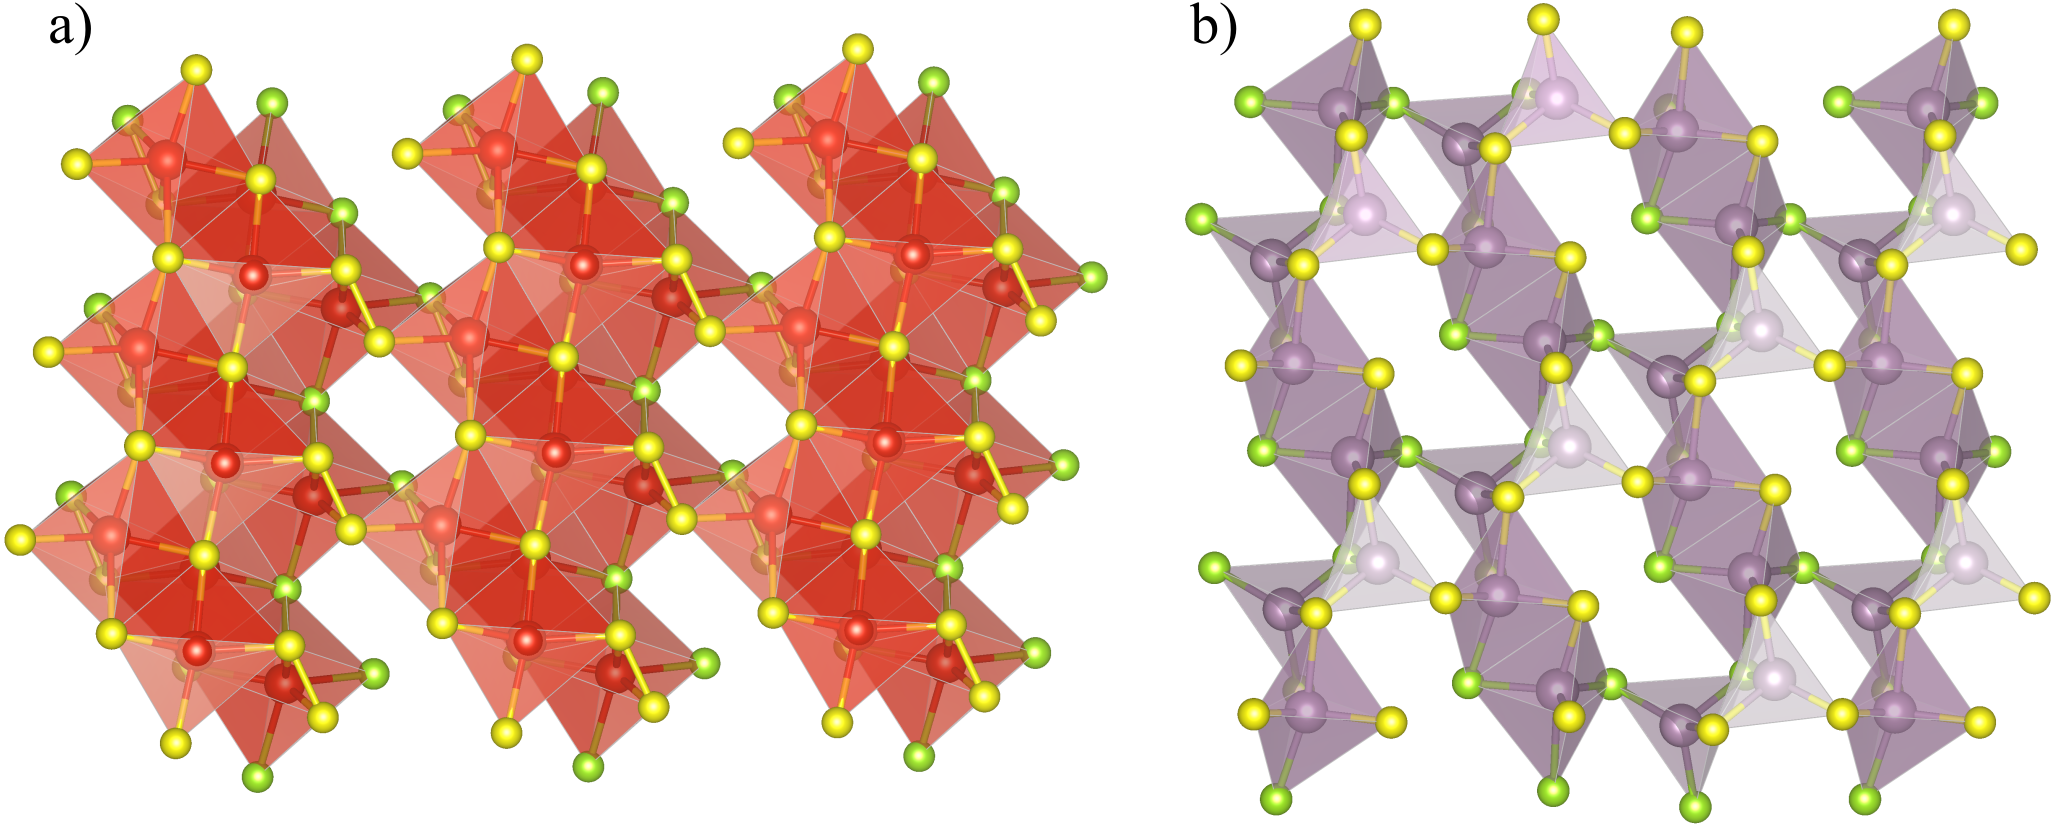
\includegraphics[width=\textwidth]{airss3_poly.png}
	\caption{Crystal structures 1A''-SVSe (a) and 1A'''-SMoSe (b) with outlined coordination polyhedra.}
	\label{airss3_poly}
\end{figure}




%%%%%%%%%%%%%%%%%%%%%%%%%%%
\subsubsection{Structures produced manually based on 1H}
%%%%%%%%%%%%%%%%%%%%%%%%%%

In this section, we consider crystal structures produced manually based on the 1H structure by the procedure which can be also used for the generation of the 1H' and 1S structures.
These structures, similarly to 1H' and 1S, can be considered as the possible structural models of grain boundaries.
As it will be shown below, enthalpies of the obtained structures are higher than the enthalpies of not only 1H, 1T, and 1T' but also of 1H' and 1S.
However, we leave their description here together with the description of 1H' and 1S, to illustrate the formation of molybdenum dimers in SMoSe structures.
Also, we would like to describe the procedure of structure generation, which can be applied for the generation of other similar structures.

To produce new structures with trigonal prismatic coordination of TM atoms, we present the structures as different fillings of the hexagonal nets of sulfur of 1H structure (Figure \ref{H-based}).
1H structure presents the most symmetric chess-board-like filling (Figure \ref{H-based}a).
The 1S structure can be also presented as the chess-board filling, but with the doubled triangular cells, having the form of rhombuses (Figure \ref{H-based}b).
After optimization, these rhombuses transform into the right squares (Figure \ref{H-based}b).
In 1H' structure, the empty rings are of two types.
The first is primitive (non-centered) triangles, and the second is face-centered hexagons consisting of six triangular rings connected through the faces (Figure \ref{H-based}c).
The optimization does not sufficiently change the forms of the empty rings, slightly deforming hexagons (Figure \ref{H-based}c).

Three new structures were produced in a similar way as it has been realized for 1H' and 1S.
Two structures have orthorhombic symmetry and one – the monoclinic.
We will designate them as 1O, 1O', and 1M'', respectively.
Structural data of SMoSe-1O, 1O', and 1M'' are given in {\it Supporting information} (Table \ref{t:str_test})
These structures are not dynamically stable for SVSe composition (Figure \ref{phon_svse}), and for SMoSe composition 1O and 1M'' are stable, while 1O' are not (Figure \ref{phon_smose}).
Enthalpies of 1O-SMoSe and 1M''-SMoSe are higher than that of  1S-SMoSe and 1H'-SMoSe on nearly 0.1 eV/fu.

We failed to produce new structures obeying the local charge balance, i.e. the structures in which each vertex of the trigonal prism is common for three prisms, as it is in 1H, 1H', and 1S.
In 1O, Ch atoms are common for two or four trigonal prisms, in 1O' and 1M'' – for two or three, or four trigonal prisms (Figure \ref{H-based}).
1M'' structure is different from the other structures in that it is characterized by the presence of trigonal prisms with two common faces, while in all other structures prisms have no more than one common face.
As it will be shown below, this is important for the formation of Mo--Mo dimers.
Optimization of 1M'' structure sufficiently affects the arrangement of sulfur atoms.
In the optimized 1M'' structure, the net of sulfur atoms looses the hexagonal symmetry (Figure \ref{H-based}f).
Mo atoms are not only in trigonal prismatic but also in quadratic coordination (Figure \ref{H-based}f).


The presence of common edges and faces of [MoO$_6$] trigonal prisms in 1H', 1S, 1O, 1O', and 1M'' structures results in shorter Mo--Mo distances in comparison with 1H structure, where prisms have only common edges.
In 1H structure, Mo atoms form a regular hexagonal net with all Mo--Mo bonds being equal to 3.25 \AA.
This bond length corresponds to the edge-sharing disposition of trigonal prisms.
In 1H', 1S, and 1O structures Mo--Mo distances for edge-sharing disposition in prisms are equal to 2.9--3.8 \AA.
For face-sharing disposition, the Mo--Mo distances is sufficiently shorter.
In 1H' and 1S structures, they are equal to 2.9 \AA, in 1O -- to 2.75 \AA\ and in 1O' -- to 2.62 \AA.
As it was mentioned, these distances are close to Mo--Mo distances in the zig-zag chains of Mo atoms in the 1T' structure (2.75 \AA).
This value is in turn equal to the shortest distance between Mo atoms in the {\it bcc} structure of pure Mo (2.72 \AA) \cite{MoV}.
1M'' structure is characterized by the sufficiently shorter Mo--Mo bond.
The distance between the adjacent Mo atoms in the dimer is equal to 2.22 \AA.
This short bond corresponds to quadruple Mo--Mo bond in Mo$_2^{4+}$ dimers, found in numerous organic molecules \cite{momo}.
Similar to organic molecules, in 1M'' structure  each molybdenum atom of Mo--Mo dimer is bound to four ligands that define almost right square (Figure \ref{test3_momo}).
Despite the relatively high enthalpy of the 1M'', its dynamic stability shows the theoretical possibility for the formation of quadruply bonded Mo$_2^{4+}$ dimers in metastable structures of TMDs.
The possibility was not considered before.

\begin{figure}[H] \centering
        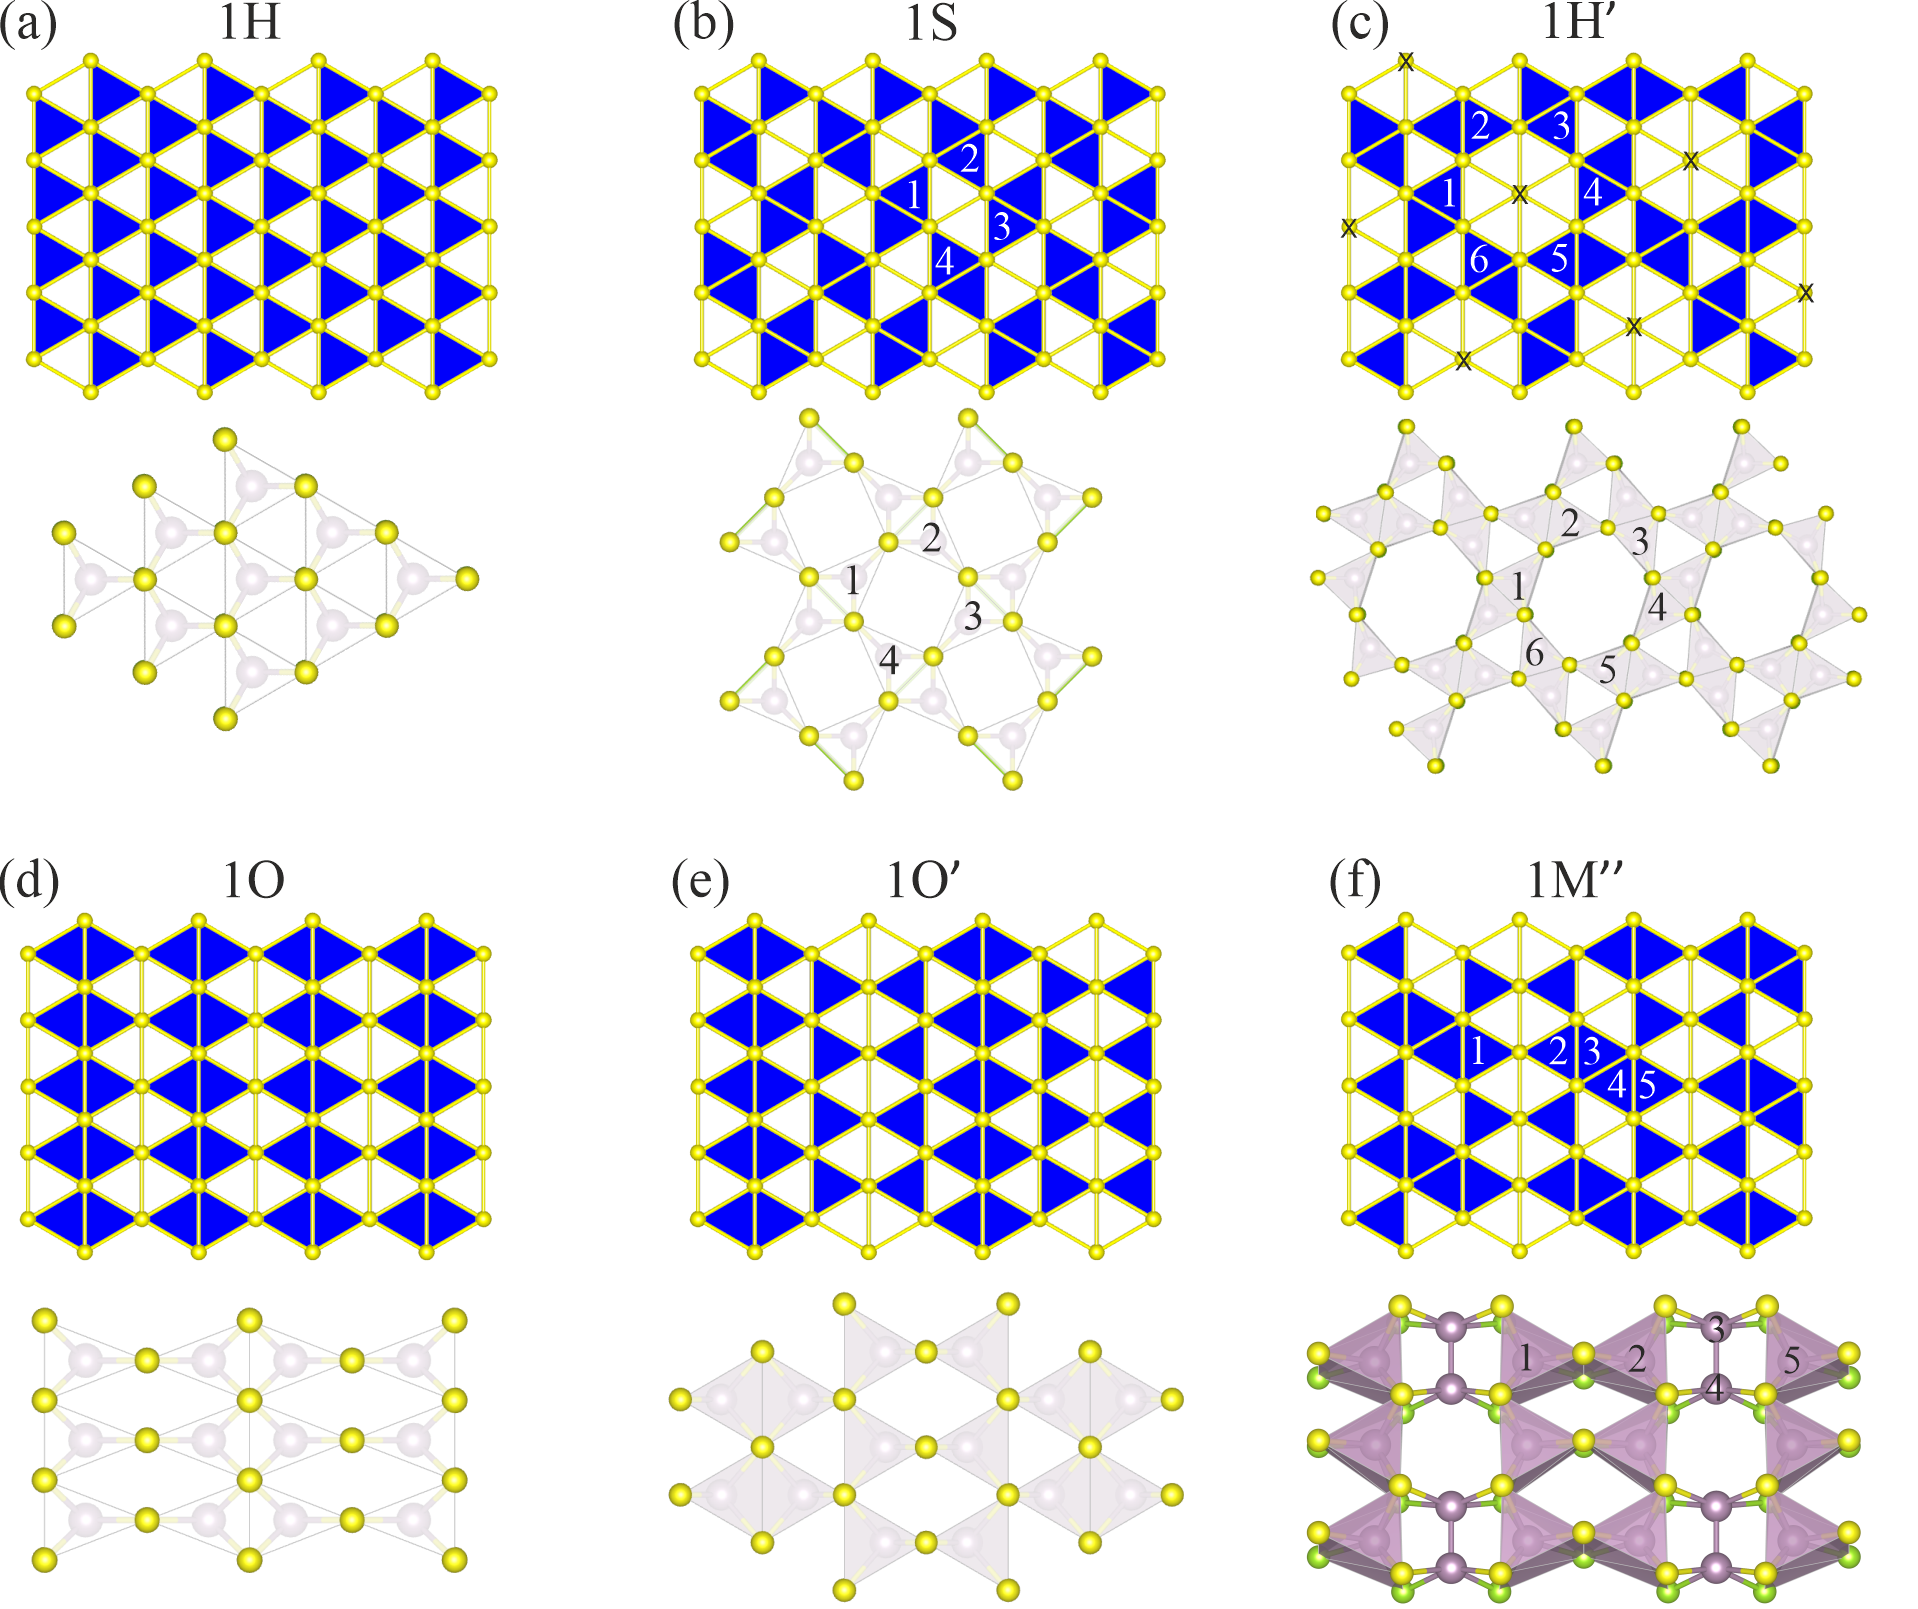
\includegraphics[width=\textwidth]{H-based.png}
        \caption{SMoSe structures produced based on 1H. Numbers on polyhedra are given to show the same fragment before and after the optimization.}
\label{H-based}
\end{figure}

\begin{figure}[H]
	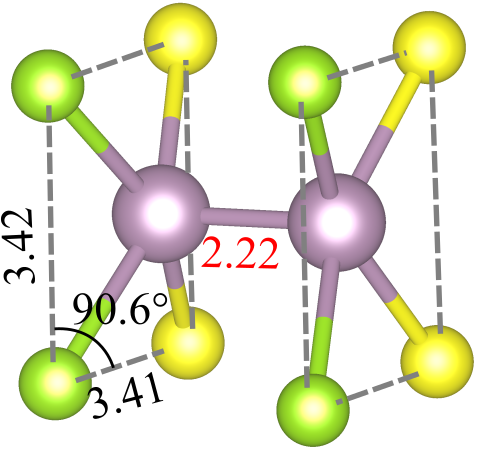
\includegraphics[width=0.3\textwidth]{test3_momo.png}
	\caption{Qadruple Mo--Mo bond in 1M''-SMoSe structure}
\label{test3_momo}
\end{figure}




%%%%%%%%%%%%%%%%%%%%%%%%
\subsection{The uniquenes of the found structures}
%%%%%%%%%%%%%%%%%%%%%%%

To answer the question, whether the found structures are unique or there are similar representatives in ICSD we have performed topological screening.
The obtained results have shown that all the found structures, except 1M', are unique and similar structures were not found in ICSD.
The same is true about the earlier known 1H' and 1S structures, similar structures of which have not also been found. 
The 1M' structure belongs to the same {\bf kgd} topological type as the 1T structure.
This means that 1M' can be transformed into the 1T without breaking the bonds.
However, the geometrical difference of 1M' and 1T structures is sufficient and transformation of one structure into the other requires changing of the coordination polyhedron from trigonal prism to the octahedron.

To evaluate the probability for the synthesis of 1A and 1A' structures on the substrate of the other compounds, we have performed the search for the structures with kagome lattices of vanadium or molybdenum atoms.
As the result, 17 structures containing flat kagome lattice of vanadium atoms and no structures with the flat lattice of molybdenum atoms have been found. 
The lengths of V--V bonds in the revealed structures vary in the range 2.43--2.81 \AA.
This is close to the lengths of bonds in the mentioned triangular clusters of Mo atoms and sufficiently higher than the lengths of V--V bonds in kagome net of 1A-SVSe.
Thus, based on the structures presented in ICSD it is problematic to suggest the proper substrate for the synthesis of 1A or 1A' structures.

It is worth noting, that ICSD is mainly the databse of experimentally syntheized 3D structures and there can be the structures synthesized in the form of monolayers or theoretically predicted structures which were not included in this database.



\subsection{Possible physical properties of the predicted structres}

As it was mentioned above, the special manuscript will be devoted to the calculations of the physical properties of the predicted structures.
Here, we would like only to speculate about the possibility of practical applications of the found structures.

The crystal field theory proceeds from the fact that the nature of ligands and their location around the central ion (symmetry of the complex) reduce the degeneracy of $d$-orbitals and change their energy. 
As all investigated structures consist of TM atoms surrounded by ligands (chalcogen atoms), the presence of the ligands splits the $d$-electrons levels depending on local symmetry.
Thereby the correlation between structure and electronic properties can be interpreted in terms of crystal field theory.
According to crystal field theory, in an octahedral environment (1T polymorph), the $d$-shell splits into a low-energy triplet (t2g) and a high-energy doublet (eg). In a trigonal prismatic geometry (1H), the low-energy triplet further splits into a doublet and a singlet [https://doi.org/10.1088/2053-1583/ab0188]. 
The two polymorphs of MoS$_2$ have distinct electronic properties, the 1H-MoS$_2$ is a semiconductor and the 1T-MoS$_2$ is metallic. The 1S-SMoSe despite the prismatic environment of TM atoms becomes a semi-metal [10.1016/j.physe.2020.114485 , 10.1039/D1NA00112D] and Mo- and W-based 1H' structures are gapless semiconductors or, alternatively, semimetals [10.1103/PhysRevB.93.035442]. 
The proposed structure airss-1 is characterized by a distorted trigonal bipyramidal local environment of the TM atom, which should make this structure more metallic due to degenerated $d$-orbitals. 
The square-pyramidal environment in airss-3 with the {\bf bare square facet} suggest the possibility for the application of this structure for molecular sorption.
\textcolor{red}{This makes materials based on these structure perspective for sensoric and catalytic uses. In addition, despite the fact that the coordination of metal atoms have a prismatic environment in the geometries 1H' and 1S make metal atoms available for use in chemical applications due to the steric factor. Смысл не ясен}

The variation of structures dictates variation of electronic properties based on different $d$-splitting and electron filling of $d$-orbitals which makes it possible to manipulate electronic properties through phase transformation.
\textcolor{blue}{Захар, надо переделать и добавить 1-2 предложения, т.к. не понятно как последнее предложение соотносится со всем текстом + последнее предложение должно быть завершающим, а тут внезапный обрыв.}



\begin{longtable}[c]{l*{9}{l}}
	\caption{Predicted structures of SMoSe and SVSe} \label{t:str}  \\
	\hline
	\multirow{2}*{Phase}	& 	\multirow{2}*{Space group}	& \multicolumn{3}{c}{\multirow{2}*{Lattice parameters (\AA, deg)}}	&	\multirow{2}*{Atom}	&	\multicolumn{3}{c}{Coordinates} \\ 
	\cline{7-9}
	&&&&&&  x	&	y	&	z \\ 
	\hline
	SVSe & $Pm\ (\#6)$  &	$a=3.6955$ & $b=12.0193$ & $c=17.1112$  & V	&	0.0921	&	0.3413	&	0.4568	\\
	&&$\alpha$ = 90.000& $\beta$=90.605& $\gamma$ = 90.000& V	&	0.5882	&	0.8456	&	0.5342	\\
	1M&&&&&	S	&	0.6057	&	0.7696	&	0.4077	\\
	&&&&&	S	&	0.0633	&	0		&	0.5125	\\
	&&&&&	S	&	0.3174	&	0.5		&	0.3765	\\
	&&&&&	Se	&	0.1058	&	0.2737	&	0.5943	\\
	&&&&&	Se	&	0.5950	&	0.5		&	0.4940	\\
	&&&&&	Se	&	0.8148	&	0		&	0.6313	\\
	\hline 
	SMoSe & $Pm\ (\#6)$  &	$a=6.2189$ & $b=3.2228$ & $c=16.7225$  & Mo	&	0.5174	&	0	&	0.5164	\\
	&   &$\alpha$ = 90.000& $\beta$=98.670& $\gamma$ = 90.000 & Mo	&	-0.0928	&	0.5	&	0.4739	\\
	1M'&&&&&   S	&	0.1525	&	0	&	0.4276	\\
	&&&&& 	S 	&	0.6730	&	0	&	0.3962	\\
	&&&&&	Se	&	0.7587	&	0.5	&	0.6054	\\
	&&&&& 	Se	&	0.2676	&	0.5	&	0.5806	\\
	\hline
	SVSe & $P1\ (\#1)$  &	$a=6.6377$ & $b=10.2914$ & $c=26.7249$  & V  &	0.1701	&	0.0669	&	0.3384	\\	
	&&$\alpha$ = 89.797& $\beta$=87.588& $\gamma$ = 89.999& V &	0.2037	&	0.5653	&	0.2917	\\
	1A &&&&&	V	&	0.6964	&	0.0669	&	0.3384	\\
	&&&&&	V	&	0.6783	&	0.5653	&	0.2917	\\
	&&&&&	V	&	0.4392	&	0.8197	&	0.3025	\\
	&&&&&	V	&	-0.0652	&	0.3195	&	0.3282	\\
	&&&&&	S	&	0.4307	&	0.6327	&	0.3525	\\
	&&&&&	S	&	0.6642	&	0.2633	&	0.3753	\\
	&&&&&	S	&	0.1896	&	0.2633	&	0.3753	\\
	&&&&&	S	&	-0.0696	&	0.5416	&	0.3542	\\
	&&&&&	S	&	0.4263	&	-0.0539	&	0.3789	\\
	&&&&&	S	&	-0.0738	&	-0.0519	&	0.3793	\\
	&&&&&	Se	&	-0.0553	&	0.1313	&	0.2699	\\
	&&&&&	Se	&	0.7136	&	0.7671	&	0.2475	\\
	&&&&&	Se	&	0.1834	&	0.7671	&	0.2475	\\
	&&&&&	Se	&	0.4450	&	0.0514	&	0.2682	\\
	&&&&&	Se	&	-0.0507	&	0.4381	&	0.2430	\\
	&&&&&	Se	&	0.4493	&	0.4438	&	0.2426	\\
	\hline 
	SMoSe & $P1\ (\#1)$  &	$a=6.5969$ & $b=9.9921$ & $c=27.6937$  & Mo  &0.1478 &0.0694  &0.3275 \\
	&&$\alpha$ = 90.024& $\beta$=87.689& $\gamma$ = 89.999& Mo &0.641 &0.116 &0.165\\
	1A'&&&&&	Mo	&	0.7221	&	0.0694	&	0.3275	\\
	&&&&&	Mo	&	0.6522	&	0.5690	&	0.3013	\\
	&&&&&	Mo	&	0.4381	&	0.8084	&	0.3090	\\
	&&&&&	Mo	&	0.9362	&	0.3069	&	0.3201	\\
	&&&&&	S	&	0.4283	&	0.6344	&	0.3668	\\
	&&&&&	S	&	0.6622	&	0.2613	&	0.3706	\\
	&&&&&	S	&	0.1931	&	0.2613	&	0.3706	\\
	&&&&&	S	&	0.9297	&	0.5373	&	0.3583	\\
	&&&&&	S	&	0.4270	&	0.9651	&	0.3745	\\
	&&&&&	S	&	0.9269	&	0.9415	&	0.3749	\\
	&&&&&	Se	&	0.9470	&	0.1309	&	0.2562	\\
	&&&&&	Se	&	0.7177	&	0.7655	&	0.2526	\\
	&&&&&	Se	&	0.1776	&	0.7655	&	0.2526	\\
	&&&&&	Se	&	0.4456	&	0.0464	&	0.2644	\\
	&&&&&	Se	&	0.9485	&	0.4613	&	0.2478	\\
	&&&&&	Se	&	0.4483	&	0.4348	&	0.2488	\\
	\hline
	SVSe & $P1\ (\#1)$  &	$a=5.0351$ & $b=8.7721$ & $c=18.0178$  & V	&	0.2426	&	-0.0280	&	0.5623	\\
	&&$\alpha$ = 77.990& $\beta$=82.386& $\gamma$ = 78.789  & V	&	0.7676	&	0.0298	&	0.4302	\\		
	1A''&&&&&	V	&	0.1205	&	0.3274	&	0.4532	\\
	&&&&&	V	&	0.8752	&	0.6755	&	0.5417	\\
	&&&&&	S	&	0.2587	&	0.0491	&	0.4287	\\
	&&&&&	S	&	0.7713	&	0.7610	&	0.4083	\\
	&&&&&	S	&	0.6782	&	0.3075	&	0.4066	\\
	&&&&&	S	&	0.1493	&	0.6174	&	0.4231	\\
	&&&&&	Se	&	0.7462	&	-0.0417	&	0.5734	\\
	&&&&&	Se	&	0.2518	&	0.2363	&	0.5951	\\
	&&&&&	Se	&	0.3271	&	0.6790	&	0.5997	\\
	&&&&&	Se	&	0.8115	&	0.3867	&	0.5779	\\
	\hline
	SMoSe & $P1\ (\#1)$  &	$a=5.8488$ & $b=7.9475$ & $c=16.7618$  & Mo	&	0.3021	&	-0.0347	&	0.5433	\\
	&&$\alpha$ = 81.296& $\beta$ = 89.766& $\gamma$ = 80.752  & Mo	&	0.6998	&	0.0412	&	0.4549	\\		
	1A'''&&&&&	Mo	&	0.0300	&	0.3220	&	0.4832	\\
	&&&&&	Mo	&	-0.0365	&	0.6754	&	0.5074	\\
	&&&&&	S	&	0.3110	&	0.1015	&	0.4123	\\
	&&&&&	S	&	0.8422	&	0.8371	&	0.3825	\\
	&&&&&	S	&	0.7777	&	0.2944	&	0.3823	\\
	&&&&&	S	&	0.2581	&	0.5193	&	0.4402	\\
	&&&&&	Se	&	0.7063	&	-0.0971	&	0.5958	\\
	&&&&&	Se	&	0.1582	&	0.1749	&	0.6229	\\
	&&&&&	Se	&	0.2359	&	0.6904	&	0.6169	\\
	&&&&&	Se	&	0.7151	&	0.4759	&	0.5584	\\
	\hline
\end{longtable}


\bibliography{2d}
\bibliographystyle{CGD}


\end{document}


Comment. 
fes structure denoted as S-MS2 in \cite{tang2021_smose}.
fxt structure denoted as H' in \cite{ma2016_h'}.
Similarly there is T' – deformed T-phase.
We can follow this notation, designating our phases by symmetry with addition of '.


2.43--2.56 -- Ta2V3Si
2.81475		-- CaV3Sb4
2.74090		--KV3Sb5
2.53143		--CoVZr
2.61895		-- Vanadium \cite{vanadium}
2.72019		-- molybdenum \cite{molybdenum}

In H-hor structure, atoms of transition metal is in trigonal prismatic coordination, similarly to 1Н structure.
The difference between 1H and H-hor structures is in that in H-hor three-folld symmetry axis of trigonal prism is parallell to the plane of the layer, while in 1H it is perpendicular.

T-hor structure is characterized by the uniqe topology– 3,3,5,8-coordinated net if short V--V bonds are considered and 3,3,5,6-coordinated net if V--V bonds are not considered.
We have not found analogues of these nets in ICSD.

among which are Ta$_2$V$_3$Si \cite{Ta2V3Si}, CaV$_3$Sb$_4$ \cite{ CaV3Sb4}, KV$_3$Sb$_5$ \cite{KV3Sb5}, and CoVZr \cite{ZrVCO}.
The structures with kagome lattice of molybdenum have not been revealed.
The structures of pure vanadium or molybdenum are characterized by the similar bond lengths, which are equal to 2.62 \AA\ \cite{MoV} and 2.72 \AA\ \cite{MoV}, respectively.

Although 1H and 1T structures are characterized by the different coordination polyhedra, they are similar in the manner of polyhedra interconnection.
The 1H structure consists of trigonal prisms [MX$_6$], and 1T structure –- of the [MX$_6$] octahedra.
Each trigonal prism share all three vertical edges with the neighbouring prisms (Figure \ref{1H1T}a); each vertex of the trigonal prism is common for two other prisms (Figure \ref{1H1T}a).
Similarly in 1T structure, each octahedron share all inclined edges with neighbouring octahedra, and no common faces; each vertex is common for three octahedra (Figure \ref{1H1T}b).
Bond valence of M--X bond is  equal to +4/6 and there are necessary three such a bonds to compensate negative charge of S$^{2-}$ anion.
Thus, local charage balance are perfectly realized in both 1H and 1T.
As it will be shown below this is not the obligatory requirement and some of the found structures does not have the local charge balance.

Only interconnection of the coordination polyhedra through the common edges is realized in 1H and 1T structure.
Below, we will show examples of the structures, with face sharing of coordination polyhedra and enthalpy lower that of 1T structure of the same composition.
